% No modificar estas líneas de código, por favor dirigirse a MARCO PRÁCTICO 

\newpage

%------------------------
%
%       MARCO PRÁCTICO
%
%------------------------



\section{MARCO DE INGENIERÍA}
En el siguiente capítulo se presenta la ingeniería del proyecto, en el cual primeramente se identifica los requerimientos necesarios para la implementación de un sistema de monitoreo remoto, el cual cuenta con una sección electrónica y programación, donde se realiza la debida evaluación y selección de componentes electrónicos, plataformas de infraestructura, entornos y lenguajes de programación.

Para esta evaluación se propone una ponderación al grado de importancia que representa el criterio en la elaboración del proyecto, además se determina un valor del 1 al 5, para cada componente dentro la selección, siendo 1 el más bajo como se observa en la \tab{val}.

\begin{tabla}[val]
{Escala de evaluación}
{Elaboración propia (2024).}
\centering
\resizebox{9cm}{!} 
{
\begin{tabular}{|c|c|} 
\hline
\rowcolor[rgb]{0.678,0.702,0.698} Valor & Descripción                           \\ 
\hline
5                                       & Cumple plenamente con el criterio.    \\
\hline
4                                       & Cumple parcialmente con el criterio.  \\
\hline
3                                       & Cumple medianamente con el criterio.  \\ 
\hline
2                                       & Cumple escasamente con el criterio.   \\ 
\hline
1                                       & No cumple con el criterio.            \\ 
\hline
\end{tabular}
}
\end{tabla}


Finalmente se realiza la suma de los productos entre la ponderación al criterio y los puntos asignados a cada componente, para así obtener el total y seleccionar el componente con el resultado más alto.

\subsection{Análisis de necesidades y requerimientos}

La empresa \acrshort{itm} requiere un sistema automatizado que permita la supervisión remota de las autoclaves en tiempo real, garantizando la seguridad, eficiencia operativa y mantenimiento preventivo. Este sistema debe facilitar la recolección de datos precisos de las variables clave (presión y temperatura) y permitir el análisis histórico de estas, generando alertas automáticas cuando se detecten valores fuera de los umbrales establecidos, este análisis se elaboró en base a entrevistas realizadas al personal de mantenimiento de la empresa \acrshort{itm}, se presenta en el Apéndice \apx{1}.

\subsubsection{Necesidades identificadas:}
\begin{itemize}
    \item Monitoreo en tiempo real de la presión y temperatura de los autoclaves desde una plataforma remota.
    \item Registro histórico de los datos monitorizados para análisis y planificación del mantenimiento preventivo.
    \item Alertas automáticas ante situaciones fuera de los parámetros operativos seguros.
    \item Acceso multiplataforma desde dispositivos móviles y de escritorio.
\end{itemize}

\subsubsection{Requerimientos del sistema}

El desarrollo del sistema debe asegurar una comunicación eficiente entre el autoclave y la nube, con acceso a la información desde una plataforma web.

\paragraph{Requerimientos a considerar para el diseño y desarrollo del proyecto}
\begin{itemize}
    \item \textbf{Monitoreo y transmisión de datos:}
    \begin{itemize}
        \item El sistema debe instalarse en las autoclaves y recoger las variables de presión y temperatura en intervalos regulares.
        \item Los datos deben transmitirse de manera confiable, segura y cifrada hacia un servidor remoto para evitar accesos no autorizados.
        \item La transmisión debe ser en tiempo real y permitir comunicación bidireccional para activar componentes o iniciar ciclos del autoclave desde la interfaz de usuario.
    \end{itemize}

    \item \textbf{Almacenamiento y gestión de datos:}
    \begin{itemize}
        \item Los datos deben ser almacenados en una base de datos centralizada que permita la consulta rápida de valores históricos y su análisis.
        \item La base de datos debe organizar la información por autoclave, permitiendo acceso a datos históricos específicos de cada equipo.
    \end{itemize}
    
    \item \textbf{Interfaz de usuario:}
    \begin{itemize}
        \item La plataforma web debe mostrar información en tiempo real de cada autoclave, con gráficas interactivas que representen la evolución de la presión, temperatura y su estado operativo.
        \item El sistema debe permitir la consulta de históricos para el análisis del rendimiento del equipo.
        \item La interfaz debe ser intuitiva y accesible desde dispositivos móviles y ordenadores, con una disposición adaptable y responsiva.
        \item Solo usuarios autorizados podrán acceder al sistema para visualizar o modificar la información, utilizando un sistema de autenticación basado en roles.
    \end{itemize}

    \item \textbf{Sistema electrónico:}
    \begin{itemize}
        \item Los componentes electrónicos del sistema de monitoreo deben estar diseñados para soportar las condiciones ambientales extremas dentro del autoclave, como alta temperatura, presión y humedad, sin comprometer su funcionamiento.
        \item La conexión entre el sistema y la autoclave debe ser confiable y resistente a posibles interferencias electromagnéticas.
    \end{itemize}
\end{itemize}

\paragraph{Requerimientos de la Autoclave}

Para asegurar el correcto funcionamiento del sistema de monitoreo, es necesario considerar los siguientes requerimientos específicos del autoclave:
\begin{itemize}
    \item \textbf{Sensores integrados:}
    \begin{itemize}
        \item Las autoclaves deben estar equipados con sensores de alta precisión para medir variables críticas como la presión y temperatura en tiempo real, con un margen de error mínimo.
    \end{itemize}

    \item \textbf{Placa de control:}
    \begin{itemize}
        \item Es necesario contar con la posibilidad de modificar la placa de control del autoclave para permitir su conexión con el sistema de monitoreo, adaptando interfaces de comunicación y protocolos para el envío y recepción de datos.
    \end{itemize}
    
    \item \textbf{Conexión a internet:}
    \begin{itemize}
        \item Las autoclaves deben poder estar conectados de forma estable a la red para garantizar que los datos de presión y temperatura puedan ser enviados al servidor de manera continua y sin interrupciones.
    \end{itemize}
\end{itemize}


\subsection{Selección de tecnología}
En esta sección se seleccionarán las tecnologías necesarias para implementar el sistema de monitoreo basado en \acrshort{iot} en el autoclave. Se evaluarán diferentes microcontroladores en función de sus características técnicas, disponibilidad y conectividad, con el fin de seleccionar el más adecuado para el proyecto.
\subsubsection{Elección del sistema electrónico}
A continuación se presenta las piezas necesarias para la implementación de la placa de monitoreo, procesamiento y envío de datos para el proyecto.
\paragraph{Microcontrolador}
El microcontrolador es una pieza clave del sistema, puesto que será el encargado de gestionar los procesos y enviar los datos a la nube. Para la elección del microcontrolador se han considerado tres opciones, que se evalúan a continuación con base en criterios de disponibilidad, capacidad de procesamiento y consumo de energía principalmente, como se muestra en la \tab{micro}.

\begin{tabla}[micro]  
{Elección del microcontrolador}
{Elaboración propia (2024).}
\centering
\resizebox{15cm}{!} 
{
\begin{tabular}{|c|c|c|c|c|c|c|c|} 
\hline
\rowcolor[rgb]{0.678,0.702,0.698} {\cellcolor[rgb]{0.678,0.702,0.698}}                                    & {\cellcolor[rgb]{0.678,0.702,0.698}}                                       & \multicolumn{2}{c|}{\textbf{ESP 32}}   & \multicolumn{2}{c|}{\textbf{ESP32-C3}} & \multicolumn{2}{c|}{\textbf{ESP-S3}}    \\
\rowcolor[rgb]{0.678,0.702,0.698} \multirow{-2}{*}{{\cellcolor[rgb]{0.678,0.702,0.698}}\textbf{CRITERIO}} & \multirow{-2}{*}{{\cellcolor[rgb]{0.678,0.702,0.698}}\textbf{PONDERACIÓN}} & \textbf{Puntos} & \textbf{Ponderación} & \textbf{Puntos} & \textbf{Ponderación} & \textbf{Puntos} & \textbf{Ponderación}  \\ 
\hline
\rowcolor[rgb]{0.027,0.894,0.698} Disponibilidad                                                          & 0.30                                                                       & 5               & 1.50                 & 4               & 1.20                 & 3               & 0.90                  \\ 
\hline
\rowcolor[rgb]{0.027,0.894,0.675} Velocidad de procesamiento                                              & 0.20                                                                       & 4               & 0.80                 & 3               & 0.60                 & 5               & 1.00                  \\ 
\hline
Seguridad                                                                                                 & 0.15                                                                       & 3               & 0.45                 & 5               & 0.75                 & 4               & 0.60                  \\ 
\hline
\rowcolor[rgb]{0.027,0.894,0.675} Consumo de energía                                                      & 0.20                                                                       & 3               & 0.60                 & 5               & 1.00                 & 4               & 0.80                  \\ 
\hline
Costo                                                                                                     & 0.15                                                                       & 4               & 0.60                 & 5               & 0.75                 & 3               & 0.45                  \\ 
\hline
\textbf{TOTAL}                                                                                            & \textbf{1}                                                                 & -               & \textbf{3.95}        & -               & \textbf{4.30}        & -               & \textbf{3.75}         \\
\hline
\end{tabular}
}
\end{tabla}
El microcontrolador seleccionado es el ESP32-C3 de la marca Seeed Studio debido a su alta disponibilidad, bajo consumo de energía y excelente conectividad, lo que lo hace ideal para el monitoreo y control remoto del autoclave en tiempo real.

\paragraph{Protocolo de red}
La elección del protocolo de red depende de los requisitos específicos del proyecto como la necesidad de comunicación en tiempo real o fiabilidad de los datos enviados, como se muestra en la \tab{red}, este nos permite realizar el envió de datos a partir de la placa de monitoreo a la nube.

\begin{tabla}[red]  
{Elección del protocolo de red}
{Elaboración propia (2024).}
\centering
\resizebox{15cm}{!} 
{
\begin{tabular}{|c|c|c|c|c|c|c|c|} 
\hline
\rowcolor[rgb]{0.678,0.702,0.698} {\cellcolor[rgb]{0.678,0.702,0.698}}                                    & {\cellcolor[rgb]{0.678,0.702,0.698}}                                       & \multicolumn{2}{c|}{\textbf{MQTT}}     & \multicolumn{2}{c|}{\textbf{WebSocket}} & \multicolumn{2}{c|}{\textbf{CoAP}}      \\
\rowcolor[rgb]{0.678,0.702,0.698} \multirow{-2}{*}{{\cellcolor[rgb]{0.678,0.702,0.698}}\textbf{CRITERIO}} & \multirow{-2}{*}{{\cellcolor[rgb]{0.678,0.702,0.698}}\textbf{PONDERACIÓN}} & \textbf{Puntos} & \textbf{Ponderación} & \textbf{Puntos} & \textbf{Ponderación}  & \textbf{Puntos} & \textbf{Ponderación}  \\ 
\hline
Consumo de energía                                                                                        & 0.15                                                                       & 5               & 0.75                 & 3               & 0.45                  & 5               & 0.75                  \\ 
\hline
\rowcolor[rgb]{0.027,0.894,0.675} Velocidad de transmisión                                                & 0.20                                                                       & 4               & 0.80                 & 5               & 1.00                  & 4               & 0.80                  \\ 
\hline
Soporte y compatibilidad                                                                                  & 0.10                                                                       & 5               & 0.50                 & 5               & 0.50                  & 4               & 0.40                  \\ 
\hline
\rowcolor[rgb]{0.027,0.894,0.675} Fiabilidad (QoS)                                                        & 0.25                                                                       & 5               & 1.25                 & 4               & 1.00                  & 3               & 0.75                  \\ 
\hline
Escalabilidad                                                                                             & 0.10                                                                       & 5               & 0.50                 & 4               & 0.40                  & 3               & 0.30                  \\ 
\hline
\rowcolor[rgb]{0.027,0.894,0.675} Seguridad                                                               & 0.20                                                                       & 5               & 1.00                 & 4               & 0.80                  & 3               & 0.60                  \\ 
\hline
\textbf{TOTAL}                                                                                            & \textbf{1}                                                                 & -               & \textbf{4.80}        & -               & \textbf{4.15}         & -               & \textbf{3.60}         \\
\hline
\end{tabular}
}
\end{tabla}
El protocolo seleccionado es \acrshort{mqtt} debido a su alta velocidad de transmisión de datos y nos permite garantizar tanto la seguridad y fiabilidad de los datos, lo que lo hace ideal para sistemas \acrshort{iot}.

\paragraph{Protocolo de comunicación de bajo nivel}
Para el desarrollo de la comunicación entre la placa de monitoreo con la autoclave se precisa garantizar una comunicación estable y segura, la elección del protocolo de comunicación de bajo nivel depende de los requisitos específicos, como consumo energético, velocidad de transmisión o fiabilidad de los datos enviados, como se presenta en la \tab{bajo}.
\begin{tabla}[bajo]  
{Elección del protocolo de comunicación de bajo nivel}
{Elaboración propia (2024).}
\centering
\resizebox{15cm}{!}
{
\begin{tabular}{|c|c|c|c|c|c|c|c|} 
\hline
\rowcolor[rgb]{0.678,0.702,0.698} {\cellcolor[rgb]{0.678,0.702,0.698}}                                    & {\cellcolor[rgb]{0.678,0.702,0.698}}                                       & \multicolumn{2}{c|}{\textbf{I2C}}      & \multicolumn{2}{c|}{\textbf{RS485}}    & \multicolumn{2}{c|}{\textbf{CAN}}       \\
\rowcolor[rgb]{0.678,0.702,0.698} \multirow{-2}{*}{{\cellcolor[rgb]{0.678,0.702,0.698}}\textbf{CRITERIO}} & \multirow{-2}{*}{{\cellcolor[rgb]{0.678,0.702,0.698}}\textbf{PONDERACIÓN}} & \textbf{Puntos} & \textbf{Ponderación} & \textbf{Puntos} & \textbf{Ponderación} & \textbf{Puntos} & \textbf{Ponderación}  \\ 
\hline
\rowcolor[rgb]{0.027,0.894,0.675} Consumo de energía                                                      & 0.20                                                                       & 5               & 1.00                 & 4               & 0.80                 & 4               & 0.80                  \\ 
\hline
\rowcolor[rgb]{0.027,0.894,0.675} Velocidad de transmisión                                                & 0.20                                                                       & 3               & 0.60                 & 4               & 0.80                 & 5               & 1.00                  \\ 
\hline
Soporte y compatibilidad                                                                                  & 0.15                                                                       & 5               & 0.75                 & 5               & 0.75                 & 3               & 0.45                  \\ 
\hline
\rowcolor[rgb]{0.027,0.894,0.675} Fiabilidad~                                                             & 0.25                                                                       & 3               & 0.75                 & 5               & 1.25                 & 5               & 1.25                  \\ 
\hline
Escalabilidad                                                                                             & 0.10                                                                       & 3               & 0.30                 & 5               & 0.50                 & 5               & 0.50                  \\ 
\hline
Costo                                                                                                     & 0.10                                                                       & 5               & 0.50                 & 4               & 0.40                 & 3               & 0.30                  \\ 
\hline
\textbf{TOTAL}                                                                                            & \textbf{1}                                                                 & -               & \textbf{3.90}        & -               & \textbf{4.50}        & -               & \textbf{4.30}         \\
\hline
\end{tabular}
}
\end{tabla}
\newpage
El protocolo seleccionado es RS485 puesto que es excelente para entornos industriales con alta tolerancia al ruido y escalabilidad, es fácil de implementar con un diseño robusto y de bajo costo por encima del protocolo \acrshort{can}.

\subsubsection{Elección de herramientas de software}
A continuación se presenta las herramientas necesarias para la implementación del sistema \acrshort{iot} tanto y su visualización en la pagina web.
\paragraph{\textit{Framework} de desarrollo web}
Los \textit{frameworks} de desarrollo web son cruciales para elaborar la aplicación web del proyecto, se requiere poder visualizar datos en tiempo real y el estados de todas las autoclaves por tanto se compara principalmente criterios de compatibilidad \acrshort{iot} y rendimiento como se presenta en la \tab{frm}.

\begin{tabla}[frm]  
{Elección del \textit{framework} de desarrollo web}
{Elaboración propia (2024).}
\centering
\resizebox{15cm}{!}
{
\begin{tabular}{|c|c|c|c|c|c|} 
\hline
\rowcolor[rgb]{0.678,0.702,0.698} {\cellcolor[rgb]{0.678,0.702,0.698}}                                    & {\cellcolor[rgb]{0.678,0.702,0.698}}                                       & \multicolumn{2}{c|}{\textbf{Next.js}}  & \multicolumn{2}{c|}{\textbf{Angular}}   \\
\rowcolor[rgb]{0.678,0.702,0.698} \multirow{-2}{*}{{\cellcolor[rgb]{0.678,0.702,0.698}}\textbf{CRITERIO}} & \multirow{-2}{*}{{\cellcolor[rgb]{0.678,0.702,0.698}}\textbf{PONDERACIÓN}} & \textbf{Puntos} & \textbf{Ponderación} & \textbf{Puntos} & \textbf{Ponderación}  \\ 
\hline
\rowcolor[rgb]{0.027,0.894,0.675} Compatibilidad con IoT                                                  & 0.25                                                                       & 5               & 1.25                 & 4               & 1.00                  \\ 
\hline
\rowcolor[rgb]{0.027,0.894,0.675} Rendimiento                                                             & 0.25                                                                       & 5               & 1.25                 & 4               & 1.00                  \\ 
\hline
Facilidad de desarrollo                                                                                   & 0.15                                                                       & 5               & 0.75                 & 3               & 0.45                  \\ 
\hline
\rowcolor[rgb]{0.027,0.894,0.675} Escalabilidad                                                           & 0.25                                                                       & 4               & 1.00                 & 5               & 1.25                  \\ 
\hline
Documentación y soporte                                                                                   & 0.10                                                                       & 4               & 0.40                 & 5               & 0.50                  \\ 
\hline
\textbf{TOTAL}                                                                                            & \textbf{1}                                                                 & -               & \textbf{4.65}        & -               & \textbf{4.20}         \\
\hline
\end{tabular}
}
\end{tabla}
\newpage
Ambos \textit{frameworks} son opciones sólidas, pero Next.js se adapta mejor al proyecto por su escalabilidad, rendimiento optimizado y compatibilidad con tecnologías \acrshort{iot}.

\paragraph{Lenguajes de programación}
Son aquellos necesarios para elaborar las aplicaciones y funcionamiento del sistema, principalmente se compara la compatibilidad con los componentes seleccionados como se presenta en la \tab{leng}.
\begin{tabla}[leng] 
{Elección de los lenguajes de programación}
{Elaboración propia (2024).}
\centering
\resizebox{15cm}{!}
{
\begin{tabular}{|c|c|c|c|c|c|c|c|} 
\hline
\rowcolor[rgb]{0.678,0.702,0.698} {\cellcolor[rgb]{0.678,0.702,0.698}}                                    & {\cellcolor[rgb]{0.678,0.702,0.698}}                                       & \multicolumn{2}{c|}{\textbf{C/C++}}    & \multicolumn{2}{c|}{\textbf{TypeScript}} & \multicolumn{2}{c|}{\textbf{Python}}    \\
\rowcolor[rgb]{0.678,0.702,0.698} \multirow{-2}{*}{{\cellcolor[rgb]{0.678,0.702,0.698}}\textbf{CRITERIO}} & \multirow{-2}{*}{{\cellcolor[rgb]{0.678,0.702,0.698}}\textbf{PONDERACIÓN}} & \textbf{Puntos} & \textbf{Ponderación} & \textbf{Puntos} & \textbf{Ponderación}   & \textbf{Puntos} & \textbf{Ponderación}  \\ 
\hline
\rowcolor[rgb]{0.027,0.894,0.698} Rendimiento                                                             & 0.30                                                                       & 5               & 1.50                 & 4               & 1.20                   & 3               & 0.90                  \\ 
\hline
\rowcolor[rgb]{0.027,0.894,0.675} Compatibilidad con IoT                                                  & 0.20                                                                       & 5               & 1.00                 & 5               & 0.80                   & 4               & 0.80                  \\ 
\hline
Documentación y soporte                                                                                   & 0.15                                                                       & 4               & 0.60                 & 5               & 0.75                   & 5               & 0.75                  \\ 
\hline
\rowcolor[rgb]{0.027,0.894,0.675} Facilidad de desarrollo                                                 & 0.20                                                                       & 3               & 0.60                 & 4               & 0.80                   & 5               & 1.00                  \\ 
\hline
Escalabilidad                                                                                             & 0.15                                                                       & 4               & 0.60                 & 5               & 0.75                   & 4               & 0.60                  \\ 
\hline
\textbf{TOTAL}                                                                                            & \textbf{1}                                                                 & -               & \textbf{4.30}        & -               & \textbf{4.30}          & -               & \textbf{4.05}         \\
\hline
\end{tabular}
}
\end{tabla}

Los lenguajes seleccionados son C/C++ para el desarrollo de la funcionalidad que tendrá el ESP32-C3 en la placa de monitoreo y TypeScript para la elaboración de la pagina web, ambos lenguajes se adaptan perfectamente a las necesidades del proyecto.

\paragraph{Broker para gestión de datos}
La elección del \textit{broker} para gestión de datos depende de la compatibilidad con el protocolo de red seleccionado, en este caso \acrshort{mqtt}, como la necesidad de comunicación en tiempo real o rendimiento es crucial para el proyecto se presenta la siguiente \tab{brk}.
\begin{tabla}[brk] 
{Elección del broker para gestión de datos}
{Elaboración propia (2024).}
\centering
\resizebox{15cm}{!}
{
\begin{tabular}{|c|c|c|c|c|c|c|c|} 
\hline
\rowcolor[rgb]{0.678,0.702,0.698} {\cellcolor[rgb]{0.678,0.702,0.698}}                                    & {\cellcolor[rgb]{0.678,0.702,0.698}}                                       & \multicolumn{2}{c|}{\textbf{Mosquitto}} & \multicolumn{2}{c|}{\textbf{EMQX}}     & \multicolumn{2}{c|}{\textbf{HiveMQ}}    \\
\rowcolor[rgb]{0.678,0.702,0.698} \multirow{-2}{*}{{\cellcolor[rgb]{0.678,0.702,0.698}}\textbf{CRITERIO}} & \multirow{-2}{*}{{\cellcolor[rgb]{0.678,0.702,0.698}}\textbf{PONDERACIÓN}} & \textbf{Puntos} & \textbf{Ponderación}  & \textbf{Puntos} & \textbf{Ponderación} & \textbf{Puntos} & \textbf{Ponderación}  \\ 
\hline
\rowcolor[rgb]{0.027,0.894,0.698} Rendimiento                                                             & 0.25                                                                       & 4               & 1.00                  & 5               & 1.25                 & 4               & 1.00                  \\ 
\hline
\rowcolor[rgb]{0.027,0.894,0.675} Compatibilidad con IoT                                                  & 0.25                                                                       & 4               & 1.00                  & 5               & 1.25                 & 5               & 1.25                  \\ 
\hline
Documentación y soporte                                                                                   & 0.15                                                                       & 4               & 0.60                  & 5               & 0.75                 & 5               & 0.75                  \\ 
\hline
\rowcolor[rgb]{0.027,0.894,0.675} Escalabilidad                                                           & 0.20                                                                       & 3               & 0.60                  & 5               & 1.00                 & 5               & 1.00                  \\ 
\hline
Facilidad de integración                                                                                  & 0.15                                                                       & 4               & 0.60                  & 5               & 0.75                 & 4               & 0.60                  \\ 
\hline
\textbf{TOTAL}                                                                                            & \textbf{1}                                                                 & -               & \textbf{3.80}         & -               & \textbf{5.00}        & -               & \textbf{4.60}         \\
\hline
\end{tabular}
}
\end{tabla}

El \textit{broker} seleccionado es EMQX por su gran rendimiento y escalabilidad sobre los demás, este nos permite gestionar de la mejor manera los datos enviados a la nube y poder realizar un análisis avanzados sobre los datos enviados.

\paragraph{Almacenamiento de datos}
Para la elección de la plataforma de almacenamiento de datos se considera el almacenamiento de datos en tiempo real, la escalabilidad y las necesidades específicas para análisis de datos de series temporales, se presenta en la tabla \tab{dat}.
\begin{tabla}[dat] 
{Elección de la base de datos}
{Elaboración propia (2024).}
\centering
\resizebox{15cm}{!}
{
\begin{tabular}{|c|c|c|c|c|c|c|c|} 
\hline
\rowcolor[rgb]{0.678,0.702,0.698} {\cellcolor[rgb]{0.678,0.702,0.698}}                                    & {\cellcolor[rgb]{0.678,0.702,0.698}}                                       & \multicolumn{2}{c|}{\textbf{MongoDb}}  & \multicolumn{2}{c|}{\textbf{Firebase}} & \multicolumn{2}{c|}{\textbf{InfluxDb}}  \\
\rowcolor[rgb]{0.678,0.702,0.698} \multirow{-2}{*}{{\cellcolor[rgb]{0.678,0.702,0.698}}\textbf{CRITERIO}} & \multirow{-2}{*}{{\cellcolor[rgb]{0.678,0.702,0.698}}\textbf{PONDERACIÓN}} & \textbf{Puntos} & \textbf{Ponderación} & \textbf{Puntos} & \textbf{Ponderación} & \textbf{Puntos} & \textbf{Ponderación}  \\ 
\hline
\rowcolor[rgb]{0.027,0.894,0.698} Datos en tiempo real                                                    & 0.25                                                                       & 4               & 1.00                 & 5               & 1.25                 & 5               & 1.25                  \\ 
\hline
\rowcolor[rgb]{0.027,0.894,0.675} Series temporales                                                       & 0.25                                                                       & 5               & 1.25                 & 3               & 0.75                 & 5               & 1.25                  \\ 
\hline
Facilidad de integración                                                                                  & 0.15                                                                       & 5               & 0.75                 & 5               & 0.75                 & 4               & 0.60                  \\ 
\hline
\rowcolor[rgb]{0.027,0.894,0.675} Escalabilidad                                                           & 0.20                                                                       & 5               & 1.00                 & 4               & 0.80                 & 4               & 0.80                  \\ 
\hline
Costo                                                                                                     & 0.15                                                                       & 4               & 0.60                 & 2               & 0.30                 & 3               & 0.45                  \\ 
\hline
\textbf{TOTAL}                                                                                            & \textbf{1}                                                                 & -               & \textbf{4.60}        & -               & \textbf{3.85}        & -               & \textbf{4.35}         \\
\hline
\end{tabular}
}
\end{tabla}
\newpage
La base de datos seleccionada es MongoDb por su disponibilidad de herramientas para \acrshort{iot} como datos en tiempo real, su gran escalabilidad para el proyecto y su facilidad de integración con la pagina web.
\paragraph{Entorno de programación}
El entorno de programación seleccionado por excelencia es Visual Studio Code para la elaboración de la pagina web, para el desarrollo del código para el ESP32-C3 se presenta los siguientes como se muestra en la \tab{ent}.
\begin{tabla}[ent] 
{Elección del entorno de programación}
{Elaboración propia (2024).}
\centering
\resizebox{15cm}{!}
{
\begin{tabular}{|c|c|c|c|c|c|c|c|} 
\hline
\rowcolor[rgb]{0.678,0.702,0.698} {\cellcolor[rgb]{0.678,0.702,0.698}}                                    & {\cellcolor[rgb]{0.678,0.702,0.698}}                                       & \multicolumn{2}{c|}{\textbf{Arduino IDE}} & \multicolumn{2}{c|}{\textbf{Platform IO}} & \multicolumn{2}{c|}{\textbf{ESP-IDF}}   \\
\rowcolor[rgb]{0.678,0.702,0.698} \multirow{-2}{*}{{\cellcolor[rgb]{0.678,0.702,0.698}}\textbf{CRITERIO}} & \multirow{-2}{*}{{\cellcolor[rgb]{0.678,0.702,0.698}}\textbf{PONDERACIÓN}} & \textbf{Puntos} & \textbf{Ponderación}    & \textbf{Puntos} & \textbf{Ponderación}    & \textbf{Puntos} & \textbf{Ponderación}  \\ 
\hline
\rowcolor[rgb]{0.027,0.894,0.698} Disponibilidad de librerías                                             & 0.30                                                                       & 4               & 1.20                    & 5               & 1.50                    & 4               & 1.20                  \\ 
\hline
\rowcolor[rgb]{0.027,0.894,0.675} Soporte para ESP32                                                      & 0.30                                                                       & 4               & 1.20                    & 5               & 1.50                    & 5               & 1.50                  \\ 
\hline
\rowcolor[rgb]{0.027,0.894,0.675} Capacidad de depuración                                                 & 0.25                                                                       & 5               & 1.25                    & 5               & 1.25                    & 5               & 1.25                  \\ 
\hline
Gestión de proyectos                                                                                      & 0.15                                                                       & 3               & 0.45                    & 5               & 0.75                    & 5               & 0.75                  \\ 
\hline
\textbf{TOTAL}                                                                                            & \textbf{1}                                                                 & -               & \textbf{4.10}           & -               & \textbf{5.00}           & -               & \textbf{4.70}         \\
\hline
\end{tabular}
}
\end{tabla}

El entorno de programación seleccionado es PlatformIO por tener el soporte para dispositivos ESP32 y gran disponibilidad de librerías para el proyecto, ademas este puede ser usado como extensión en Visual Studio Code.
\paragraph{Herramienta de diseño electrónico}
En la siguiente \tab{disel} se presenta las herramientas disponibles para diseñar la placa \acrshort{pcb} del sistema de monitoreo y operación, el cual principalmente se compara los componentes disponibles en el \textit{software}.
\begin{tabla}[disel] 
{Elección de la herramienta de diseño electrónico}
{Elaboración propia (2024).}
\centering
\resizebox{15cm}{!}
{
\begin{tabular}{|c|c|c|c|c|c|c|c|} 
\hline
\rowcolor[rgb]{0.678,0.702,0.698} {\cellcolor[rgb]{0.678,0.702,0.698}}                                    & {\cellcolor[rgb]{0.678,0.702,0.698}}                                       & \multicolumn{2}{c|}{\textbf{EasyEDA}}  & \multicolumn{2}{c|}{\textbf{Kicad}}    & \multicolumn{2}{c|}{\textbf{Proteus}}   \\
\rowcolor[rgb]{0.678,0.702,0.698} \multirow{-2}{*}{{\cellcolor[rgb]{0.678,0.702,0.698}}\textbf{CRITERIO}} & \multirow{-2}{*}{{\cellcolor[rgb]{0.678,0.702,0.698}}\textbf{PONDERACIÓN}} & \textbf{Puntos} & \textbf{Ponderación} & \textbf{Puntos} & \textbf{Ponderación} & \textbf{Puntos} & \textbf{Ponderación}  \\ 
\hline
\rowcolor[rgb]{0.027,0.894,0.675} Interfaz                                                                & 0.20                                                                       & 5               & 1.00                 & 4               & 0.80                 & 4               & 0.80                  \\ 
\hline
\rowcolor[rgb]{0.027,0.894,0.675} Componenetes                                                            & 0.30                                                                       & 5               & 1.50                 & 4               & 1.20                 & 3               & 0.90                  \\ 
\hline
Diseño PCB                                                                                                & 0.15                                                                       & 4               & 0.60                 & 4               & 0.60                 & 5               & 0.75                  \\ 
\hline
\rowcolor[rgb]{0.027,0.894,0.675} Simulación~                                                             & 0.25                                                                       & 4               & 1.00                 & 5               & 1.25                 & 5               & 1.25                  \\ 
\hline
Costo                                                                                                     & 0.10                                                                       & 5               & 0.50                 & 4               & 0.40                 & 3               & 0.30                  \\ 
\hline
\textbf{TOTAL}                                                                                            & \textbf{1}                                                                 & -               & \textbf{4.60}        & -               & \textbf{4.25}        & -               & \textbf{4.00}         \\
\hline
\end{tabular}

}

\end{tabla}

El \textit{software} seleccionado es EasyEDA, por su gran disponibilidad de componentes actualizados y su interfaz de usuario que ofrece facilidad para desarrollar el diseño \acrshort{pcb} y simulación, ademas al ser una herramienta \textit{online} no hay necesidad de descargar ningún \textit{software} adicional.

\subsection{Diseño del proyecto}
En la presente sección se explica el proceso de diseño del proyecto en base a los requerimientos y necesidades.
\subsubsection{Diseño electrónico}
Una vez seleccionados los componentes electrónicos se presenta el proceso del diseño del sistema electrónico, el cual fue basado en el diagrama de bloques mostrado en la Figura \ref{fig:siselec}.
\begin{figure}[!htb]
    \centering
    \caption{Diagrama de bloques del sistema electrónico} % Título de figura
    {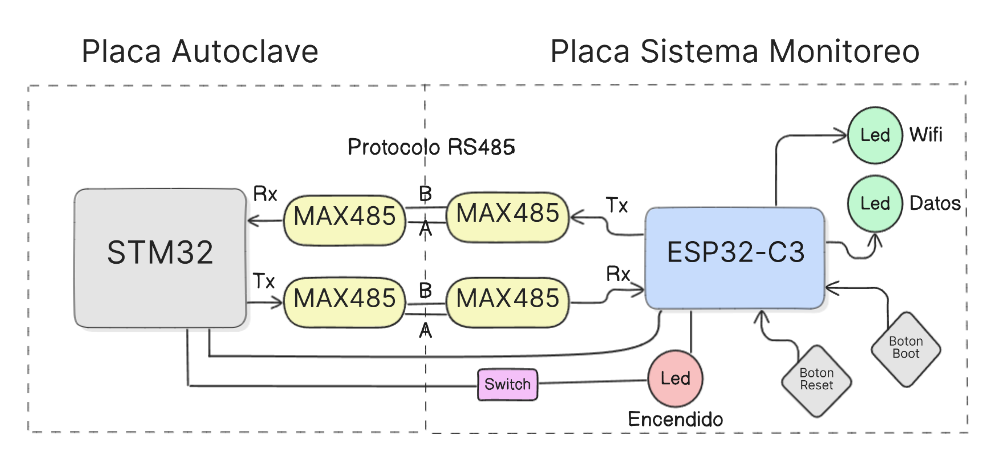
\includegraphics[width=0.9\columnwidth]{Figuras/siselec.png}}\\
    \centering{\textbf{Fuente:} Elaboración propia (2024)} % Fuente
    \label{fig:siselec}
\end{figure}
\newpage
Para la elaboración de los diagramas electrónicos se utilizó el \textit{software} EasyEDA. El diseño electrónico está compuesto por:
\begin{itemize}
    \item Conexión de microcontrolador.
    \item Conexión de comunicación RS485.
    \item Placa \acrshort{pcb}.
\end{itemize}

\paragraph{Conexión de microcontrolador}
El microcontrolador seleccionado es el Seeed Studio XIAO ESP32C3 enfocado en tecnologías \acrshort{iot}, según el diseño presentado el microcontrolador estará conectado a los siguientes componentes electrónicos:
\begin{itemize}
    \item Primer \acrshort{led}: Indicador de alimentación.
    \item Segundo \acrshort{led}: Indicador de conexión a \acrshort{wifi}.
    \item Tercer \acrshort{led}: Indicador de envío o recepción de datos.
    \item Botones: El primer botón para \textit{reset} y el segundo para \textit{boot} del microcontrolador.
    \item Interruptor: Encargado de permitir el paso de alimentación a la placa de monitoreo proveniente de la placa de control de la autoclave.
    \item UART: Conexión a los componentes MAX485.
\end{itemize}
En la siguiente Figura \ref{fig:esp32dia} se presenta el respectivo diagrama de conexión del microcontrolador a los demás componentes electrónicos, el diagrama completo se presenta en el Apéndice \apx{2}:
\begin{figure}[!htb]
    \centering
    \caption{Diagrama de conexión microcontrolador} % Título de figura
    {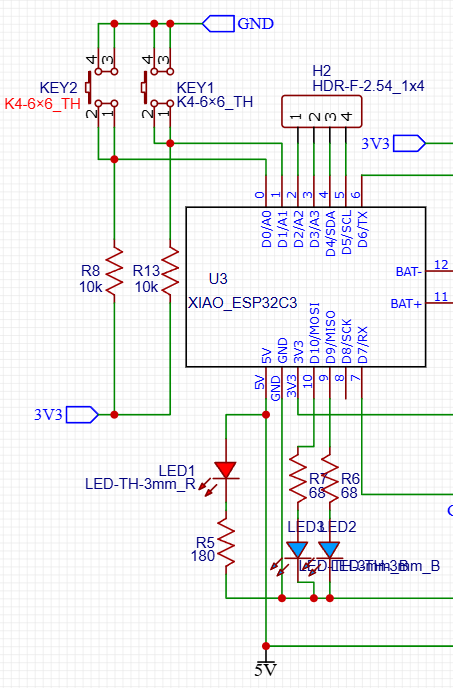
\includegraphics[width=0.5\columnwidth]{Figuras/esp32dia.png}}\\
    \centering{\textbf{Fuente:} Elaboración propia (2024)} % Fuente
    \label{fig:esp32dia}
\end{figure}
\paragraph{Conexión de comunicación RS485}
Para el diseño de ambas placas de control, se decidió implementar dos integrados MAX485, uno para transmisión y otro par recepción, de esta manera se garantiza la comunicación bidireccional de ambas partes, el diseño propuesto se muestra en la siguiente Figura \ref{fig:maxdia}, el diagrama completo se presenta en el Apéndice \apx{2}.
\begin{figure}[!htb]
    \centering
    \caption{Diagrama de protocolo de comunicación RS485} % Título de figura
    {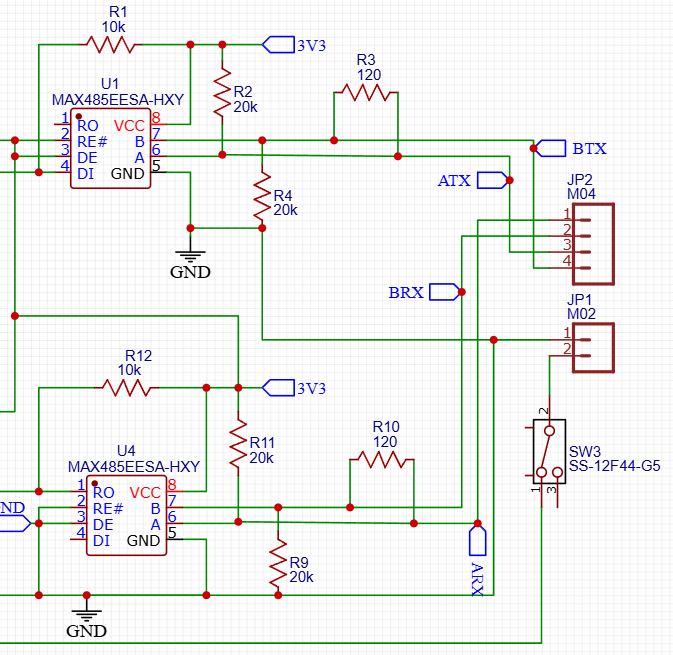
\includegraphics[width=0.6\columnwidth]{Figuras/max485dia.png}}\\
    \centering{\textbf{Fuente:} Elaboración propia (2024)} % Fuente
    \label{fig:maxdia}
\end{figure}

\paragraph{Placa PCB}
Utilizando la herramienta EasyEDA y a partir del diagrama elaborado, se genera el diseño de la placa \acrshort{pcb} para el proyecto. Se busca llegar a un diseño compacto y de reducido tamaño, por tanto los componentes a elegir son del tipo \acrfull{smd}, en la siguiente Figura \ref{fig:pistas} se muestra el diseño final de la placa. 
\begin{figure}[!htb]
    \centering
    \caption{Diagrama \acrshort{pcb}} % Título de figura
    {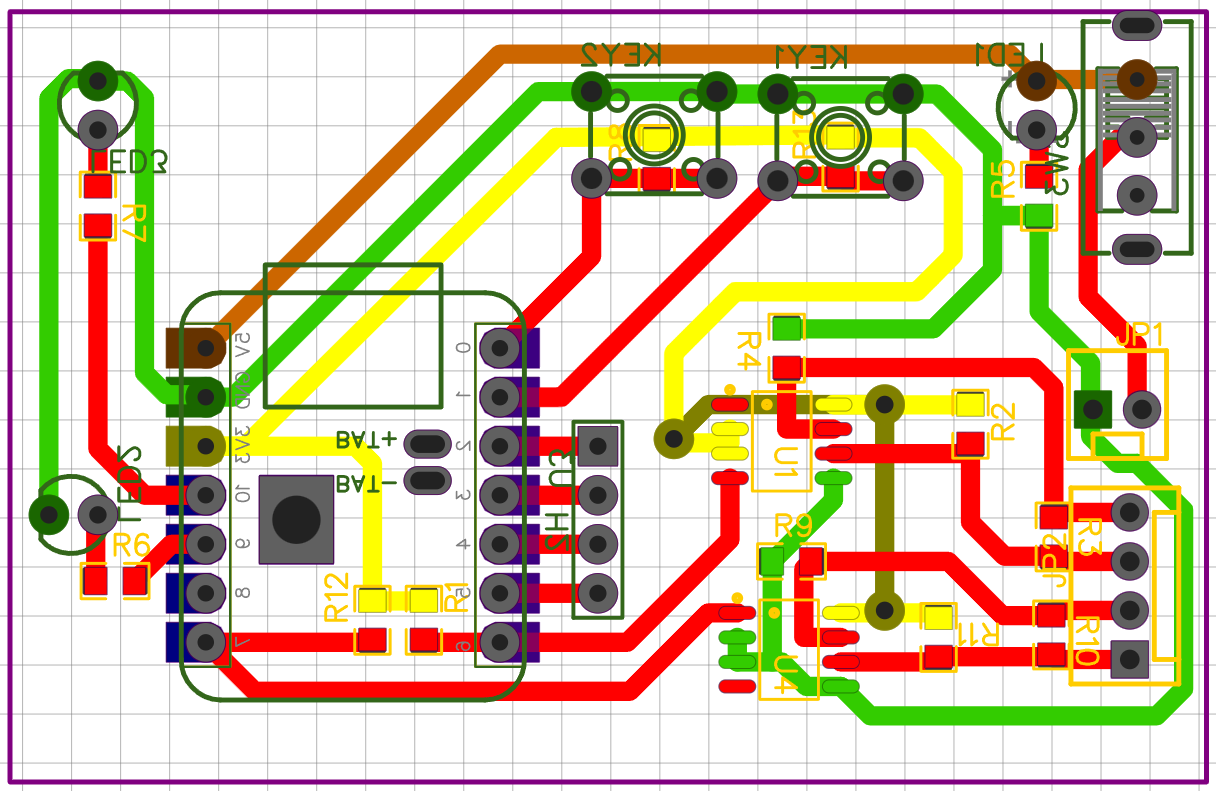
\includegraphics[width=0.8\columnwidth]{Figuras/pistas.png}}\\
    \centering{\textbf{Fuente:} Elaboración propia (2024)} % Fuente
    \label{fig:pistas}
\end{figure}
\newpage
Para finalizar, se presenta el modelo 3d de la placa \acrshort{pcb} en la Figura \ref{fig:3d} para tener mejor dimensionamiento al realizar el diseño mecánico.
\begin{figure}[hpt]
    \centering
    % Título de figura
    \caption{Modelo 3d de la placa \acrshort{pcb}}
        % imagen 1
        \subfloat[Vista superior]{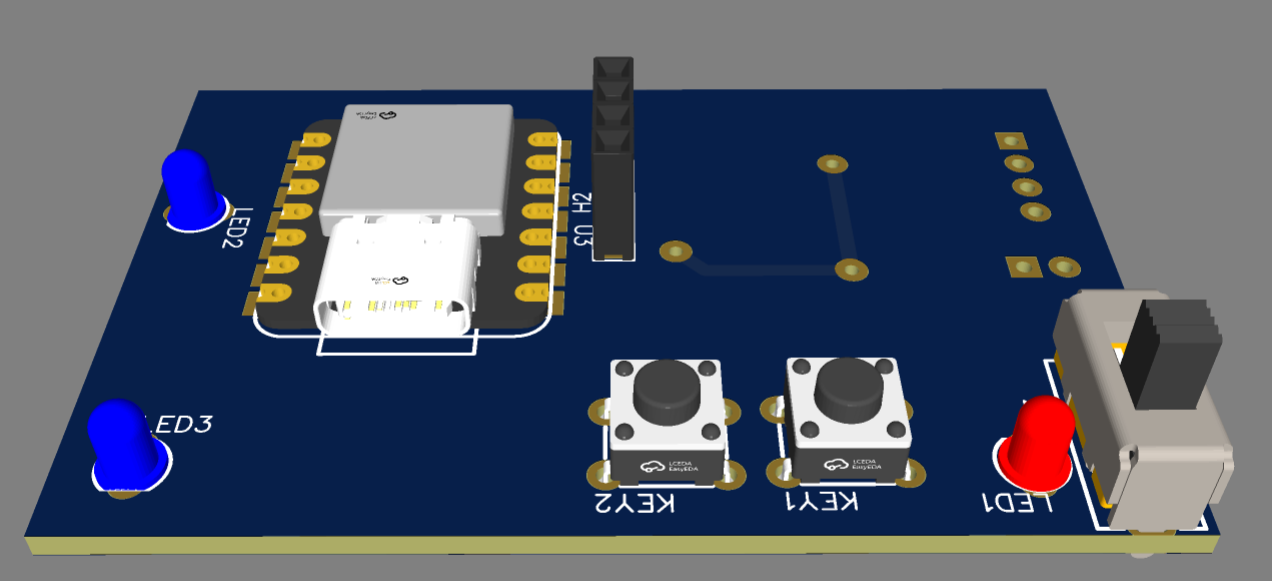
\includegraphics[width=0.45\columnwidth]{Figuras/pcb3d1.png}}
        % separaciones | agregar una de las opciones entre cada par de imágenes
            \qquad      % figuras en la misma linea
            %\par        % siguiente línea
        % imagen 2
        \subfloat[Vista inferior]{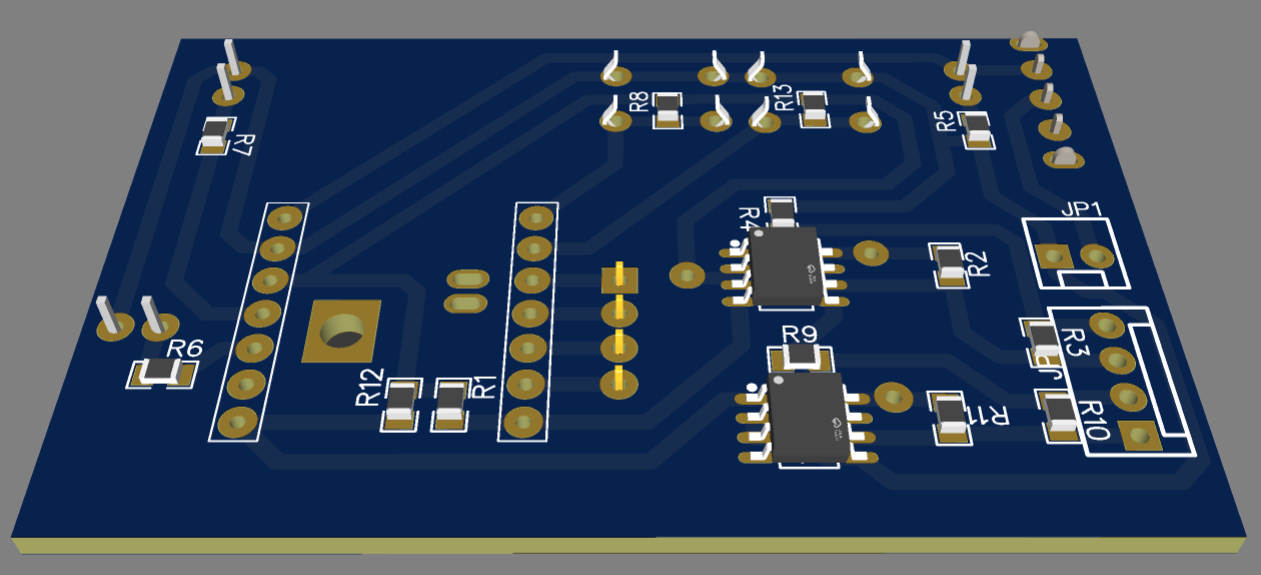
\includegraphics[width=0.45\columnwidth]{Figuras/pcb3d2.png}}\\
    \centering{\textbf{Fuente:} Elaboración propia (2024)}
    \label{fig:3d}
\end{figure}

\subsubsection{Diseño de la arquitectura funcional del sistema de monitoreo}
Para esta sección se debe detallar cada elemento dentro del sistema de monitoreo que permita recopilar y enviar los datos extradidos de la autoclave había la nube y posteriormente ser almacenado en la base de datos, una vez ya seleccionada la tecnología a utilizar dentro del proyecto se puede observar la conexión de la misma en la siguiente Figura \ref{fig:arqui}.
\begin{figure}[!htb]
    \centering
    \caption{Diagrama arquitectónico del sistema} % Título de figura
    {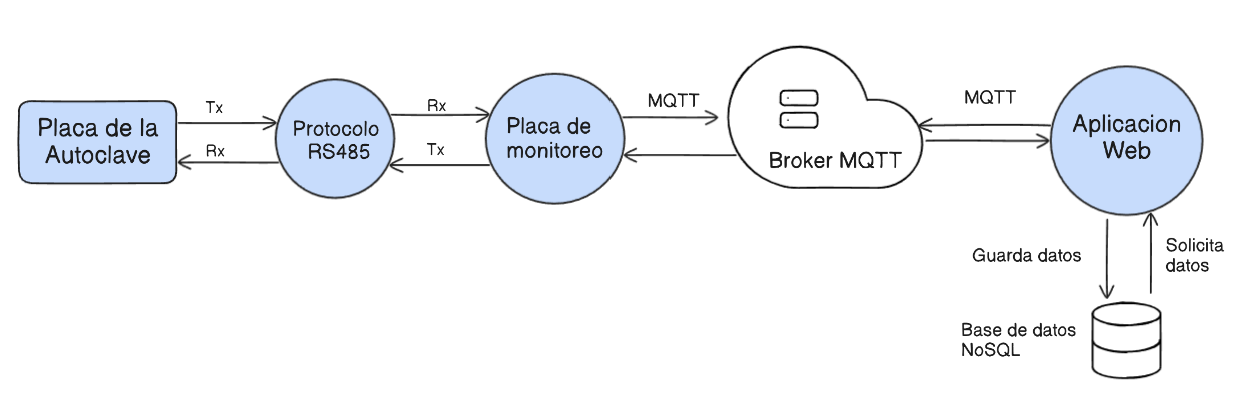
\includegraphics[width=1\columnwidth]{Figuras/arqui.png}}\\
    \centering{\textbf{Fuente:} Elaboración propia (2024)} % Fuente
    \label{fig:arqui}
\end{figure}

A continuación se detalla el proceso que sigue funcionamiento del ESP32-C3 en el Apéndice \apx{3}.

\subsubsection{Diseño de la pagina web}
En base a los requerimientos y necesidades de la empresa y del sistema se plantea las siguientes ventanas a ser implementadas en la aplicación web: 
\begin{itemize}
    \item Principal: Bienvenida al usuario.
    \item \textit{Login}: Ingreso de credenciales del usuario.
    \item \textit{Dashboard}: Datos generales sobre todas las autoclaves de la empresa.
    \item Vista para cada autoclave
    \item Control Manual: Para operar cada elemento individual de la autoclave.
    \item Control Automático: Para iniciar un ciclo y observar resultados.
    \item Reportes: Datos históricos de procesos almacenados anteriormente.
    \item Conexiones: Datos sobre la conexión \acrshort{wifi} y su configuración.
    \item Información: Datos a cerca la autoclave.
\end{itemize}

\subsubsection{Diseño mecánico}
El diseño mecánico involucra el diseño \acrshort{cad} y \acrshort{cae} para la carcasa de la placa del sistema de monitoreo, fue realizado con el \textit{software} de SolidWorks. Además, se contempla un diseño compacto y resistente, adaptado para soportar las condiciones operativas sin comprometer la funcionalidad de la placa.
\paragraph{Diseño CAD}
El diseño se compone de dos piezas elaboradas para la carcasa como se puede apreciar en la siguiente Figura \ref{fig:case}, cuenta con una tapa superior e inferior que encajan entre sí.
\begin{figure}[hpt]
    \centering
    % Título de figura
    \caption{Carcasa de la placa de monitoreo}
        % imagen 1
        \subfloat[Tapa superior]{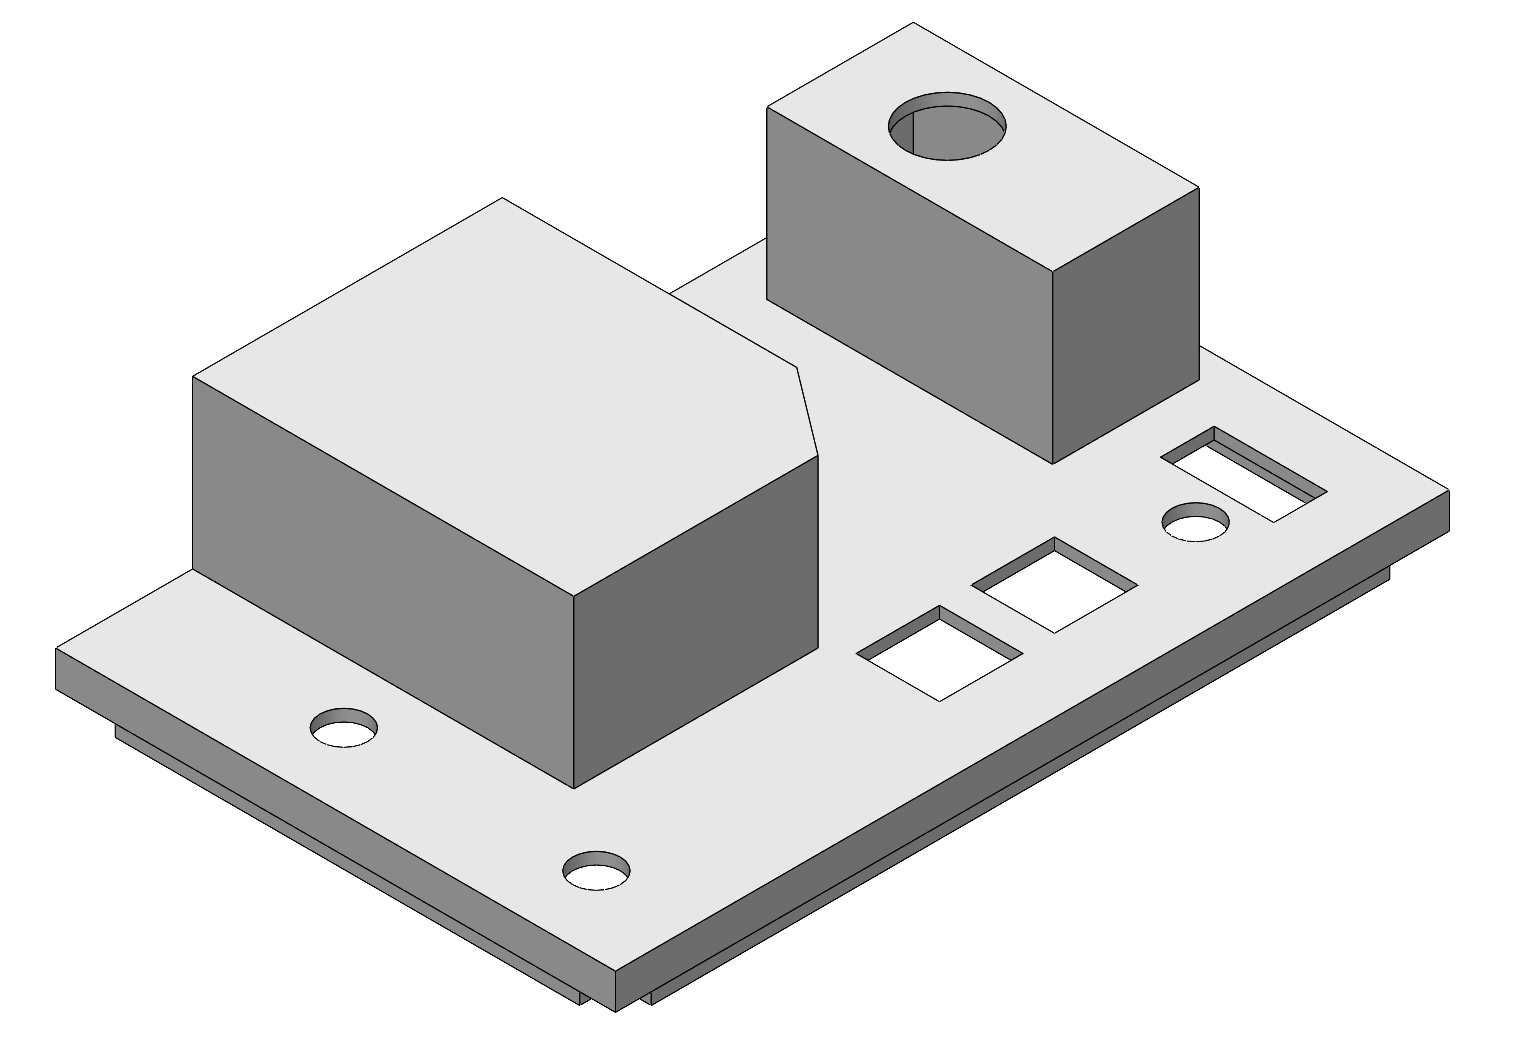
\includegraphics[width=0.45\columnwidth]{Figuras/tapa1.png}}
        % separaciones | agregar una de las opciones entre cada par de imágenes
            \qquad      % figuras en la misma linea
            %\par        % siguiente línea
        % imagen 2
        \subfloat[Tapa inferior]{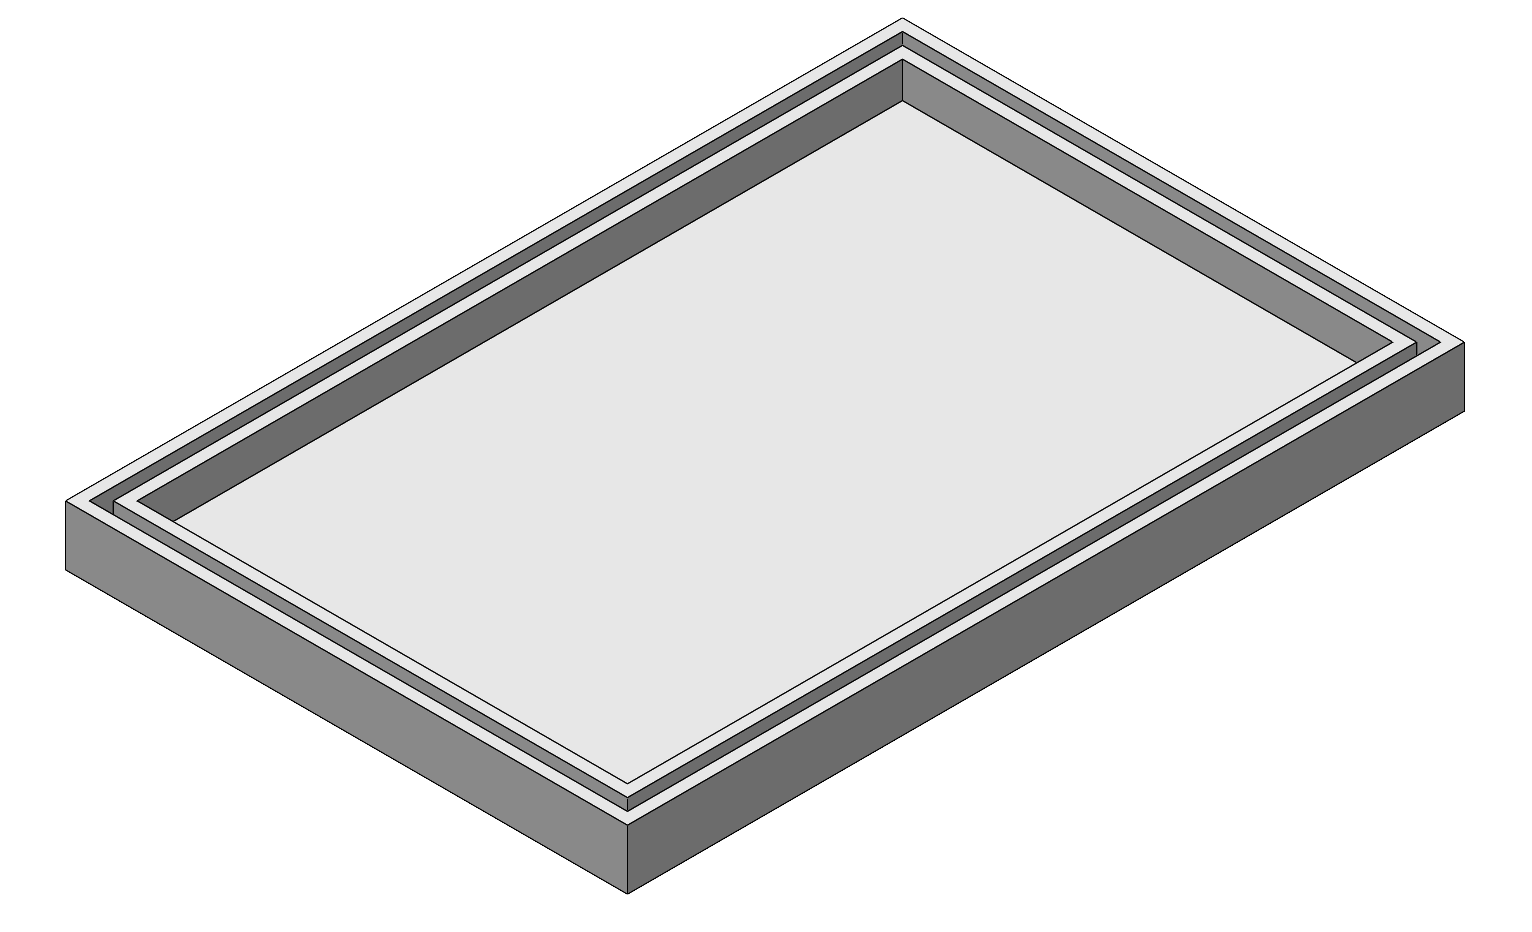
\includegraphics[width=0.45\columnwidth]{Figuras/tapa2.png}}\\
    \centering{\textbf{Fuente:} Elaboración propia (2024)}
    \label{fig:case}
\end{figure}

Para el ensamblaje del prototipo se importaron los componentes electrónicos seleccionados para el proyecto y componentes mecánicos como se observa en la Figura \ref{fig:ensam}.
\begin{figure}[!htb]
    \centering
    \caption{Ensamblaje} % Título de figura
    {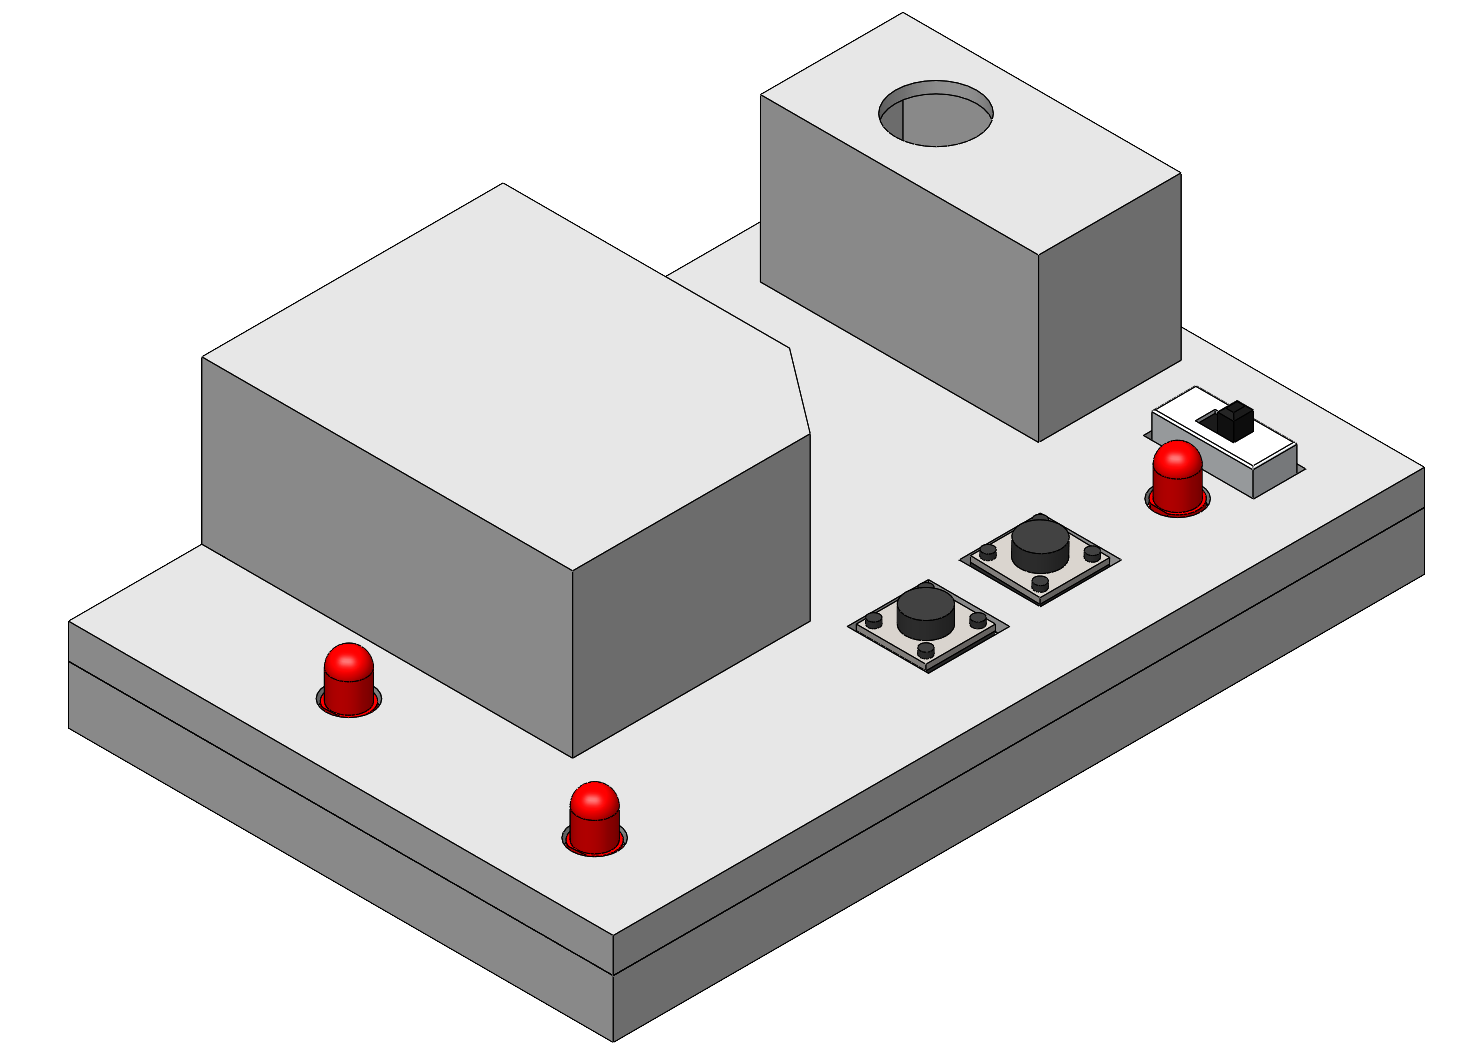
\includegraphics[width=0.8\columnwidth]{Figuras/ensam.png}}\\
    \centering{\textbf{Fuente:} Elaboración propia (2024)} % Fuente
    \label{fig:ensam}
\end{figure}
\newpage
Los componentes fueron ensamblados en sus respectivas posiciones dando lugar a un margen de error, no se toma en cuenta otros artículos de ensamblaje (Tornillos, Pernos) puesto que ambas tapas fueron diseñadas con su respectivo apriete mecánico. Los planos mecánicos se encuentran el Apéndice \apx{4}.

\paragraph{Diseño CAE}
Mediante el \textit{software} SolidWorks se realizaron estudios de esfuerzo y desplazamiento sobre las piezas.

La carcasa soporta el peso de la placa de monitoreo mas los cables de conexión a la placa de control de la autoclave, por lo que se encuentra sometido a una carga de 15 [g] por parte de la placa y 20 [g] de los cables, repartiendo el peso entre el soporte de cables recibe una fuerza 0,1962 [N] y la base de la carcasa con una fuerza de 0,14715 [N], como se observa en la Figura \ref{fig:cargas}. El material elegido para la carcasa es \acrfull{pla}.

\begin{figure}[!htb]
    \centering
    \caption{Fuerzas sobre la carcasa} % Título de figura
    {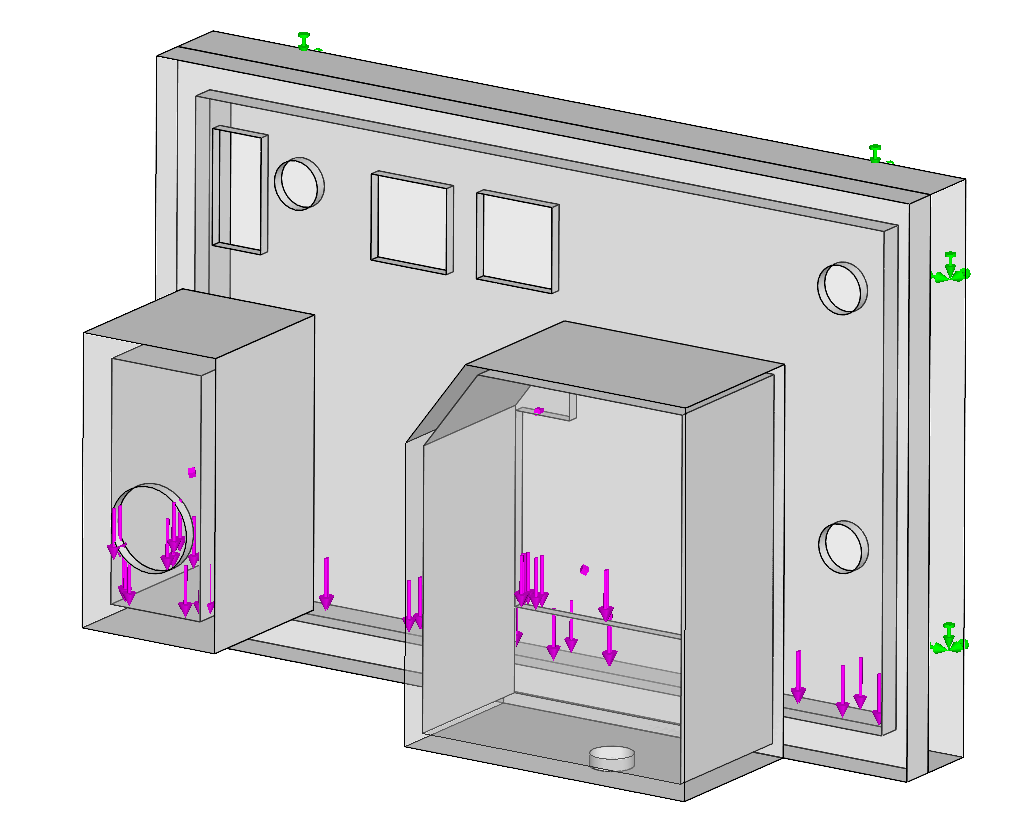
\includegraphics[width=0.8\columnwidth]{Figuras/cargas.png}}\\
    \centering{\textbf{Fuente:} Elaboración propia (2024)} % Fuente
    \label{fig:cargas}
\end{figure}

En la figura \ref{fig:simu}, puede observarse los análisis de la simulación, obteniendo los siguientes resultados:
\begin{itemize}
    \item Tensión de Von Mises mínima de 0,01769 [MPa] y máxima de 74.72 [MPa].
    \item Desplazamiento máximo de 0,000391 [mm].
\end{itemize}
\begin{figure}[hpt]
    \centering
    % Título de figura
    \caption{Resultados de simulación}
        % imagen 1
        \subfloat[Tensión]{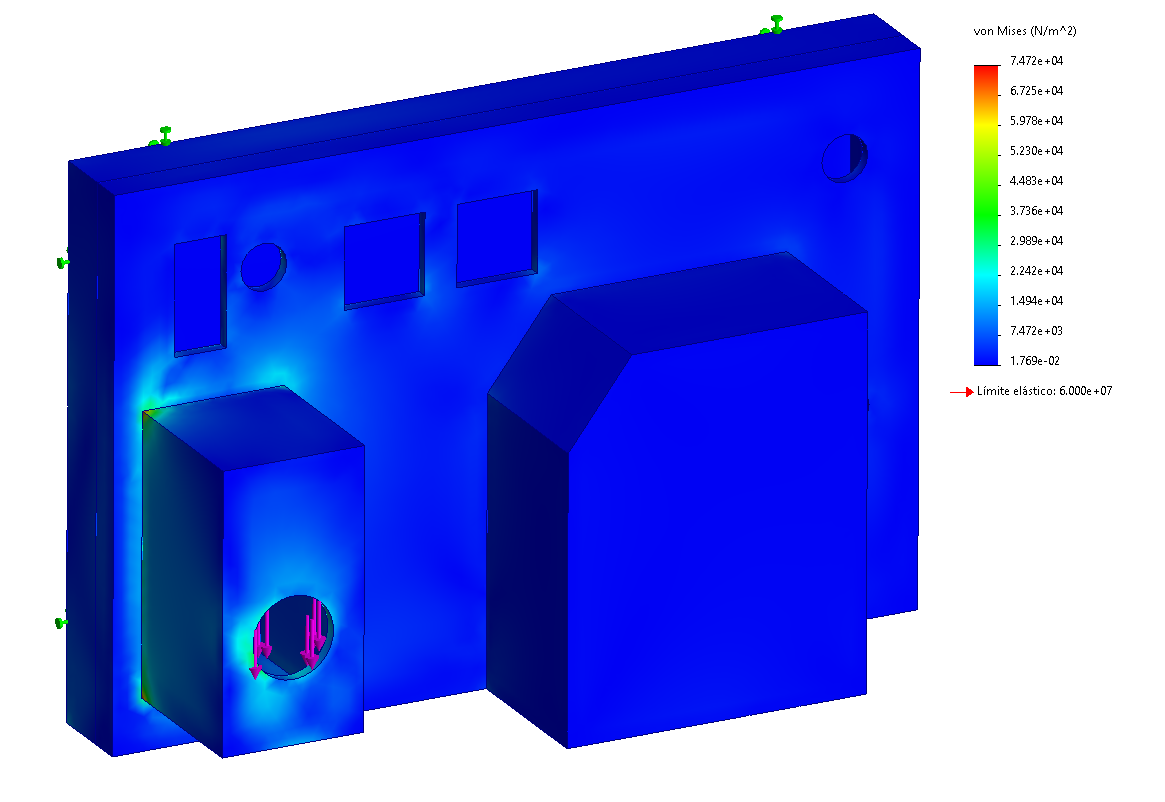
\includegraphics[width=0.47\columnwidth]{Figuras/tension.png}}
        % separaciones | agregar una de las opciones entre cada par de imágenes
            \qquad      % figuras en la misma linea
            %\par        % siguiente línea
        % imagen 2
        \subfloat[Desplazamiento]{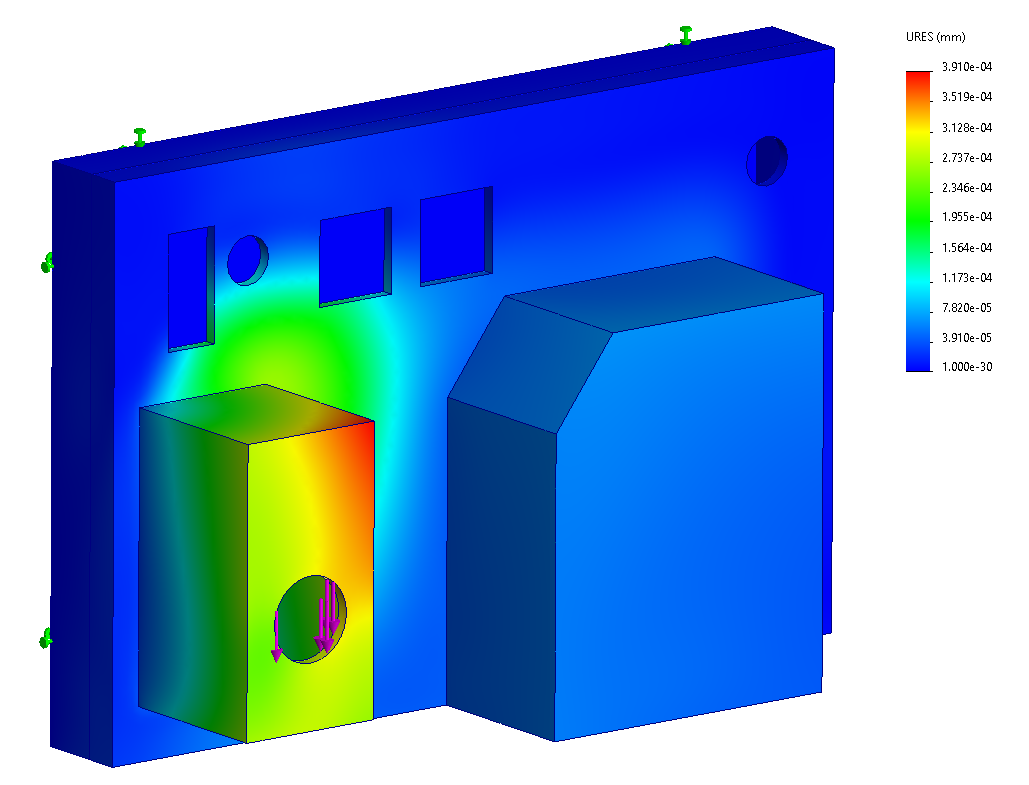
\includegraphics[width=0.45\columnwidth]{Figuras/desp.png}}\\
    \centering{\textbf{Fuente:} Elaboración propia 2024}
    \label{fig:simu}
\end{figure}
\newpage
\subsection{Implementación de sistemas}
En esta sección presentamos la implementación de los diseños propuestos.
\subsubsection{Implementación electrónica}
En base a los diseños y diagramas realizados, se implemento la respectiva placa \acrshort{pcb} del sistema de monitoreo.
\paragraph{Placa PCB}
Para la elaboración de la placa \acrshort{pcb} primeramente se imprime el diseño en una hoja de papel transfer para poder imprimir el diseño en una placa de cobre, posteriormente la dejamos remojar en cloruro férrico para eliminar el cobre sobrante como se aprecia en la siguiente Figura \ref{fig:pcbelab}.
\begin{figure}[hpt]
    \centering
    % Título de figura
    \caption{Elaboración de la placa PCB}
        % imagen 1
        \subfloat[Impresión]{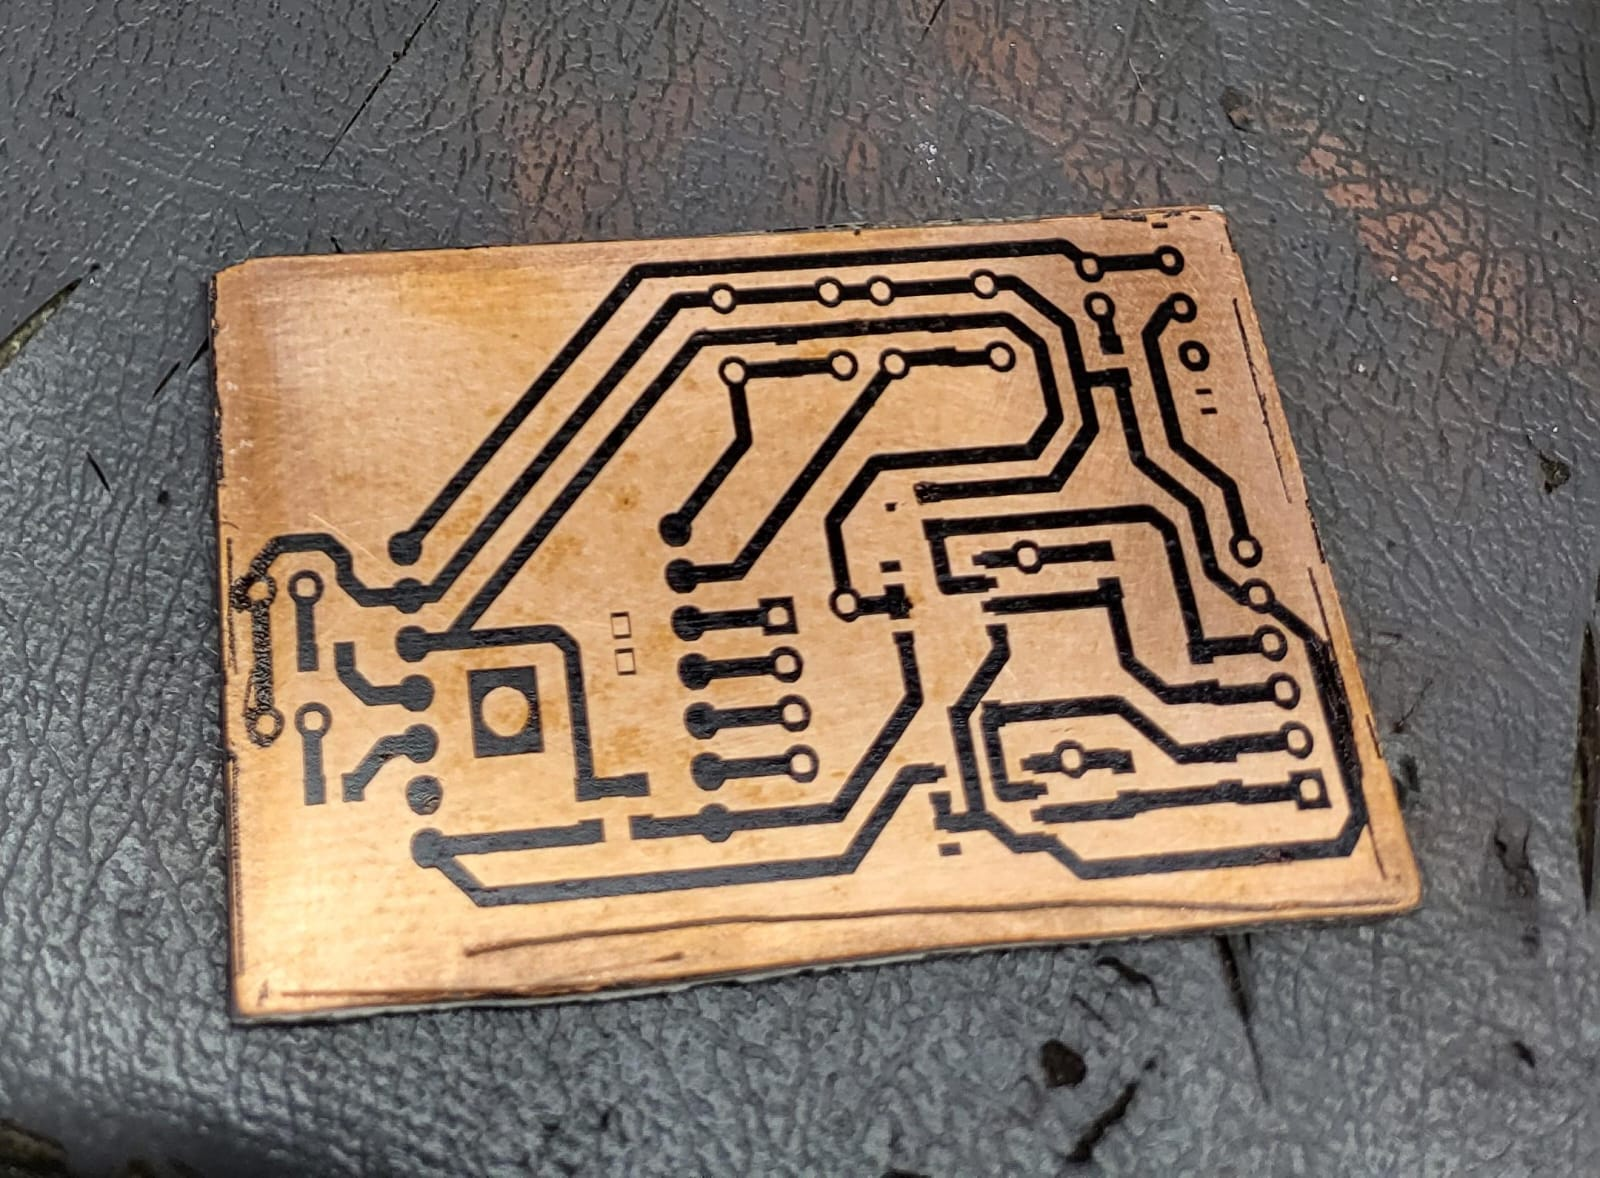
\includegraphics[width=0.45\columnwidth]{Figuras/implementacion/pcb1.jpg}}
        % separaciones | agregar una de las opciones entre cada par de imágenes
            \qquad      % figuras en la misma linea
            %\par        % siguiente línea
        % imagen 2
        \subfloat[Grabado]{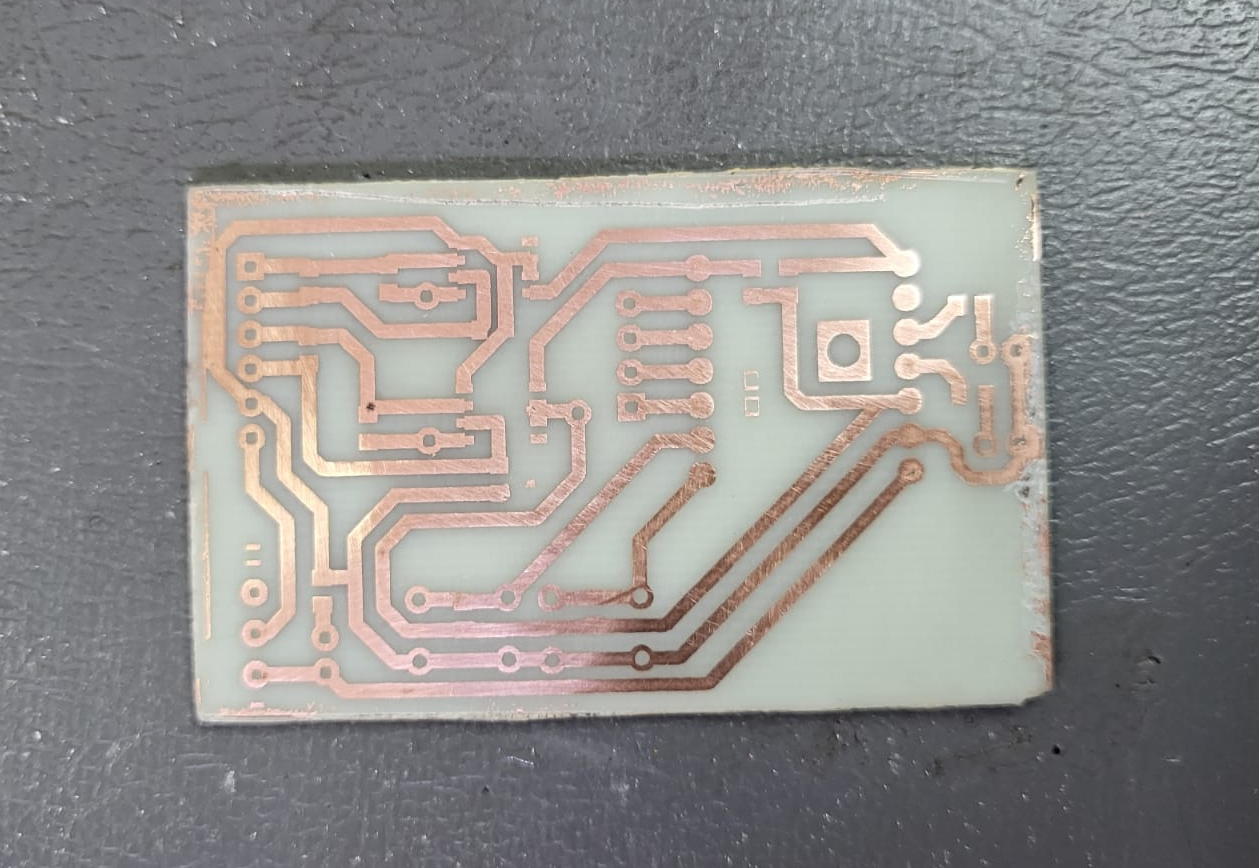
\includegraphics[width=0.45\columnwidth]{Figuras/implementacion/pcb2.png}}\\
    \centering{\textbf{Fuente:} Elaboración propia 2024}
    \label{fig:pcbelab}
\end{figure}
\newpage
A continuación se pasa a soldar los componentes seleccionados en la placa \acrshort{pcb} teniendo como resultado la Figura \ref{fig:pcbfin}.
\begin{figure}[hpt]
    \centering
    % Título de figura
    \caption{Componentes soldados a la placa}
        % imagen 1
        \subfloat[Vista inferior]{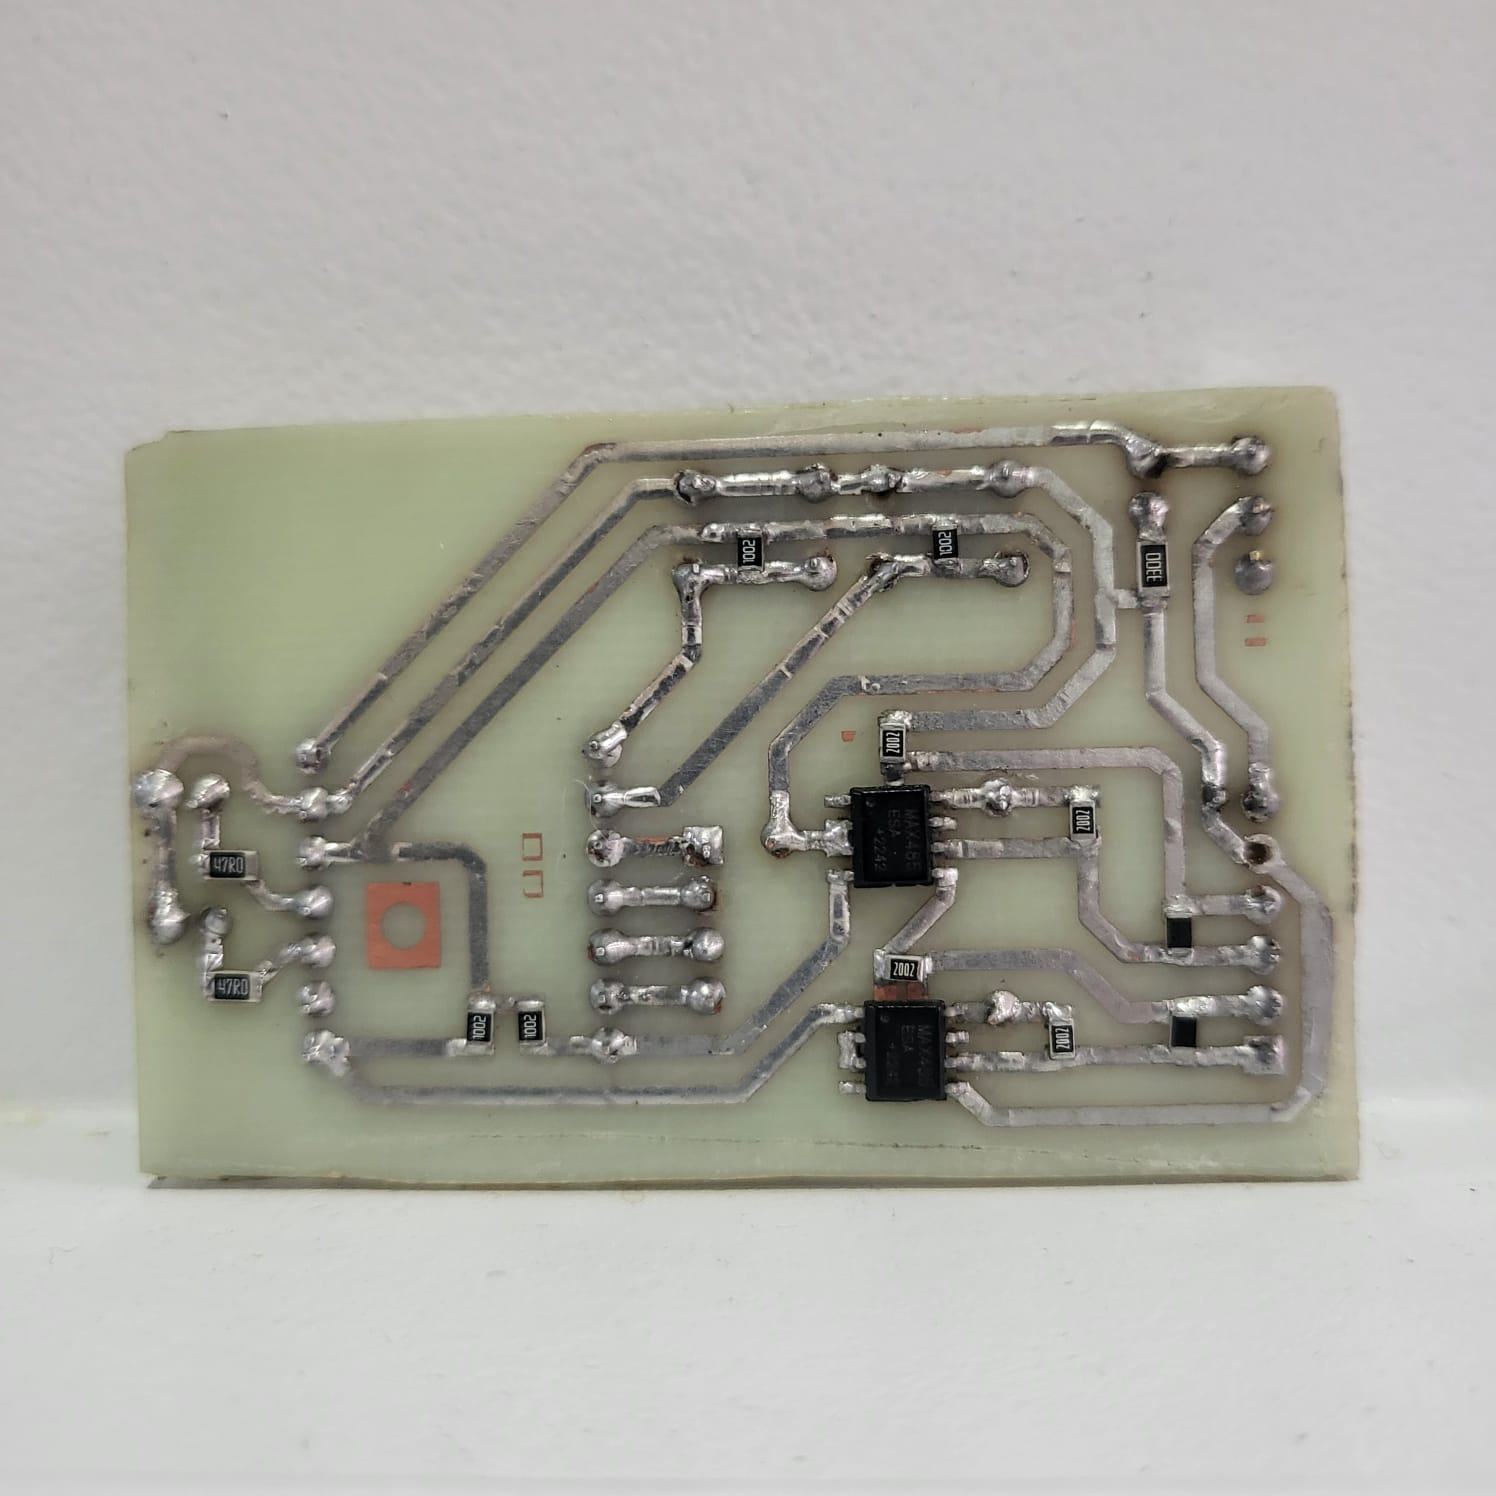
\includegraphics[width=0.4\columnwidth]{Figuras/implementacion/pcb3.jpg}}
        % separaciones | agregar una de las opciones entre cada par de imágenes
            \qquad      % figuras en la misma linea
            %\par        % siguiente línea
        % imagen 2
        \subfloat[Vista superior]{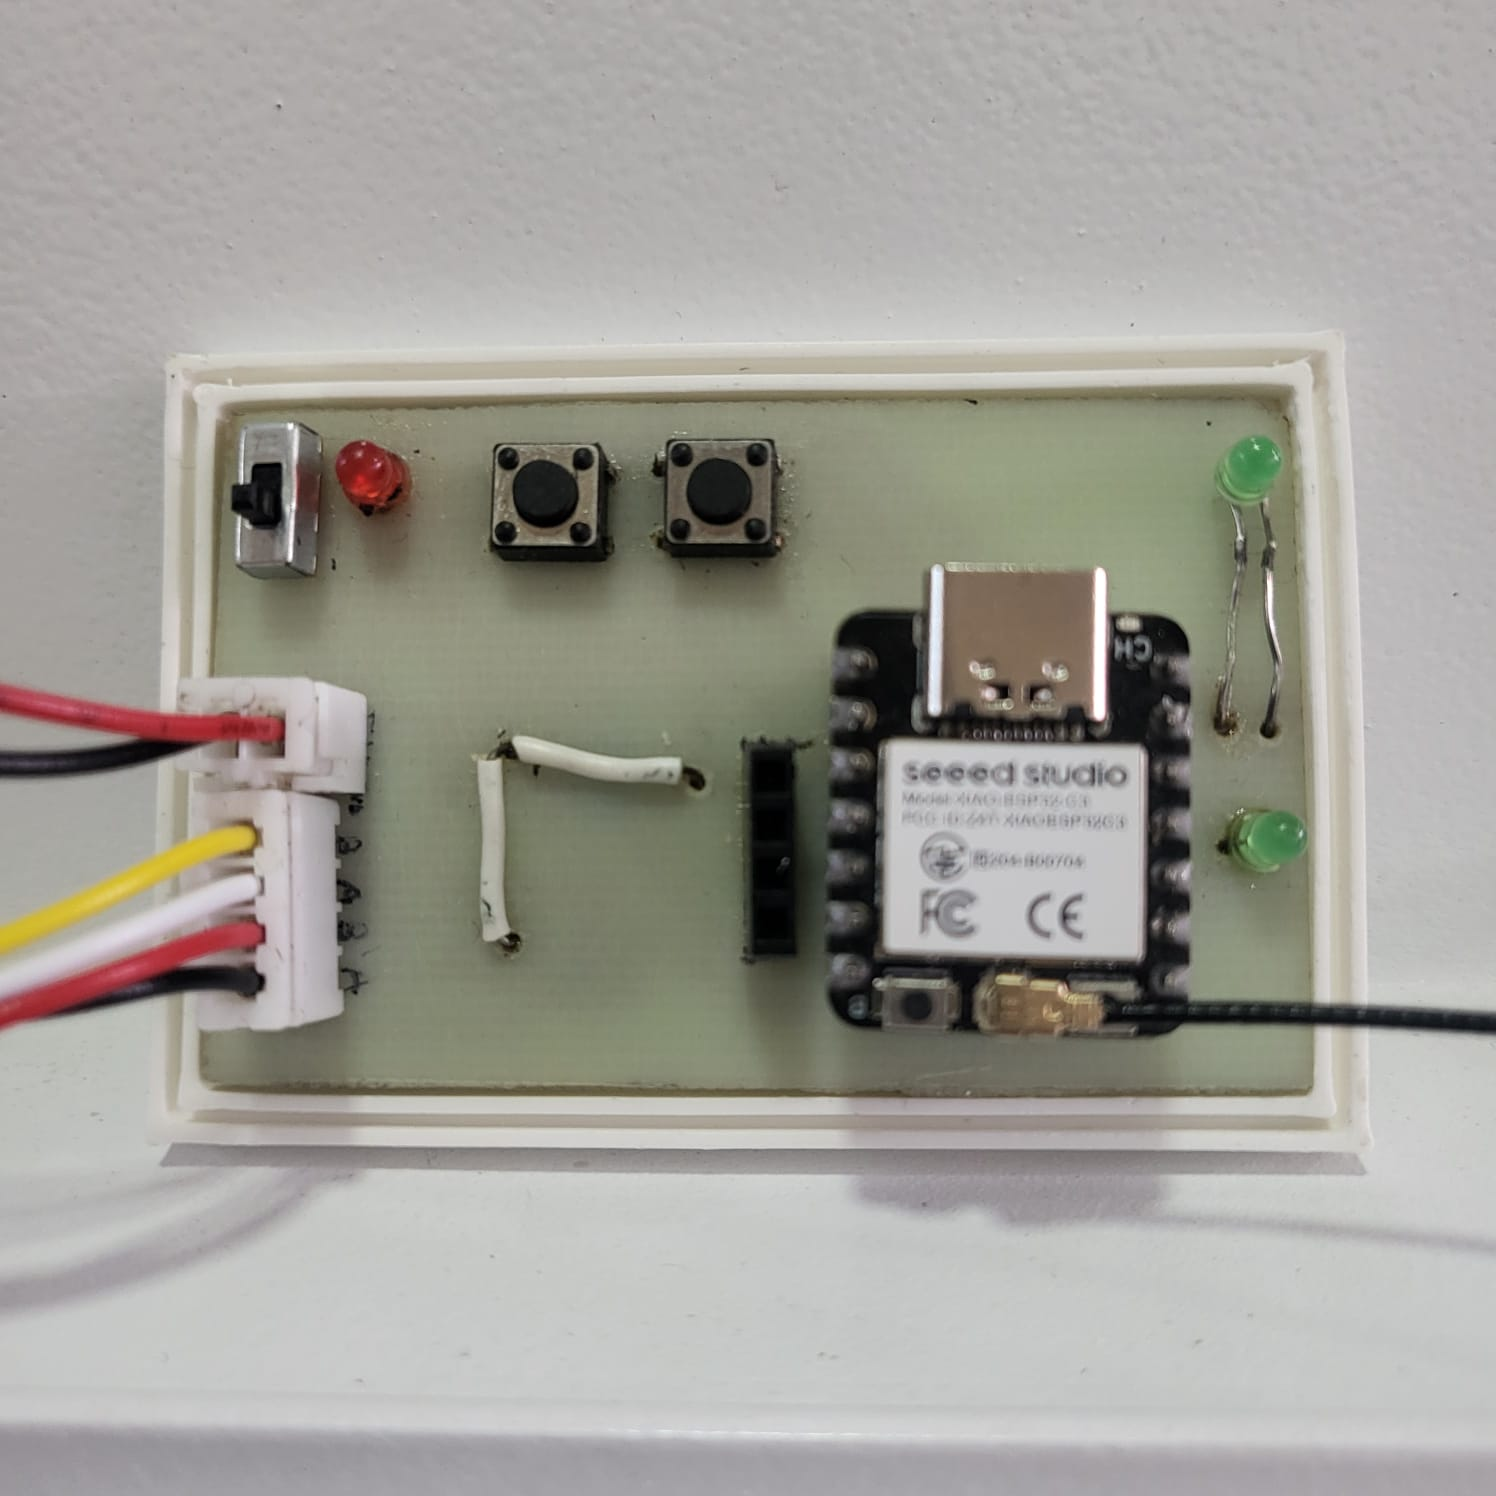
\includegraphics[width=0.4\columnwidth]{Figuras/implementacion/pcb4.jpg}}\\
    \centering{\textbf{Fuente:} Elaboración propia (2024)}
    \label{fig:pcbfin}
\end{figure}
\newpage
\subsubsection{Implementación de software}
Según el diseño propuesto se implementaron las siguientes ventanas en la aplicación web.

\textbf{Página principal:} Aquella que sirve para dar la bienvenida al usuario y dar información de la empresa Figura \ref{fig:prin}.
\begin{figure}[!htb]
    \centering
    \caption{Página principal} % Título de figura
    {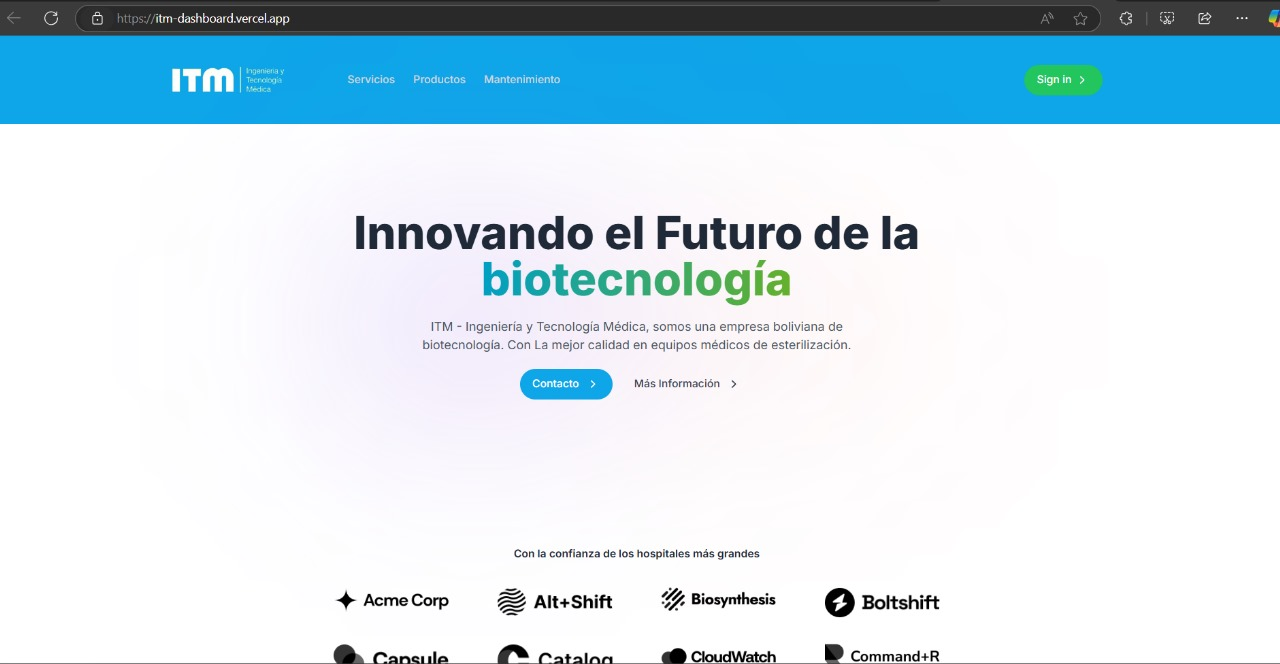
\includegraphics[width=0.8\columnwidth]{Figuras/7.jpg}}\\
    \centering{\textbf{Fuente:} Elaboración propia (2024)} % Fuente
    \label{fig:prin}
\end{figure}\\
\textbf{Login:} Lugar de ingreso de credenciales del usuario para poder acceder al sistema, la sistema de autenticación validara si es una cuenta administrador o cliente para su debida redirección Figura \ref{fig:log}.
\begin{figure}[!htb]
    \centering
    \caption{Página login} % Título de figura
    {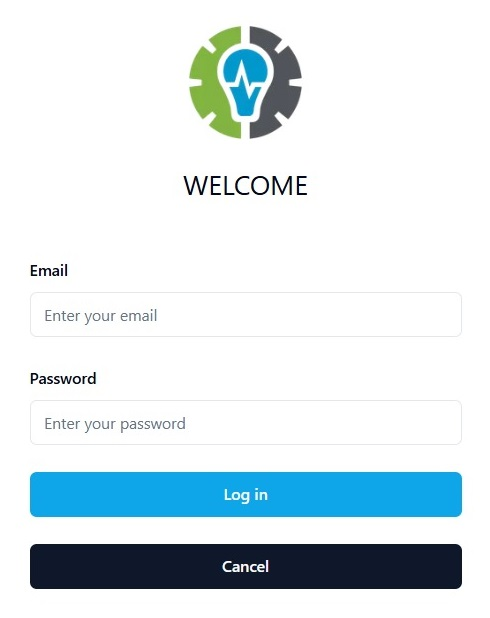
\includegraphics[width=0.5\columnwidth]{Figuras/4.jpg}}\\
    \centering{\textbf{Fuente:} Elaboración propia (2024)} % Fuente
    \label{fig:log}
\end{figure}
\newpage
\textbf{Dashboard:} Esta página presenta una tabla donde se muestran todas las autoclaves de la empresa y su respectivo estado, como tambien datos generales de cantidad y fallas. En la tabla se tiene la capacidad de acceder a cada autoclave o eliminarla Figura \ref{fig:dash}.
\begin{figure}[!htb]
    \centering
    \caption{Página dashboard} % Título de figura
    {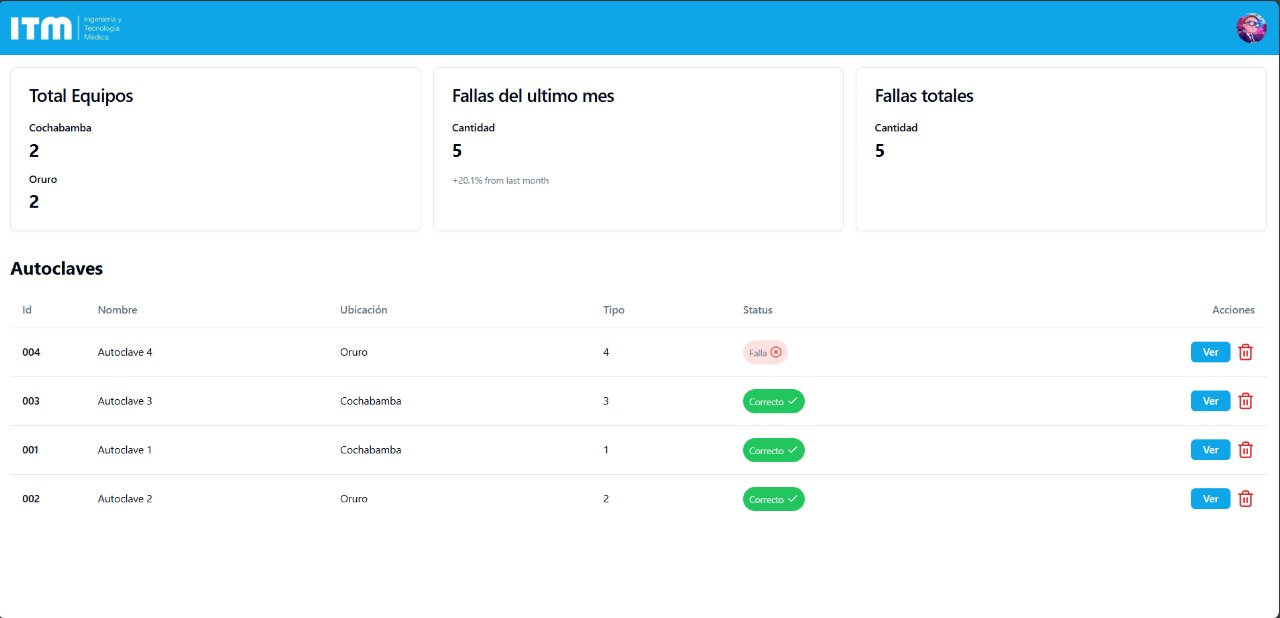
\includegraphics[width=0.9\columnwidth]{Figuras/6.jpg}}\\
    \centering{\textbf{Fuente:} Elaboración propia (2024)} % Fuente
    \label{fig:dash}
\end{figure}
\newpage
\textbf{Control Manual:} La página de acuerdo al tipo de autoclave presenta sus diferentes sensores o actuadores para poder comenzar con el control manual de cada uno de ellos Figura \ref{fig:man}.
\begin{figure}[!htb]
    \centering
    \caption{Control Manual} % Título de figura
    {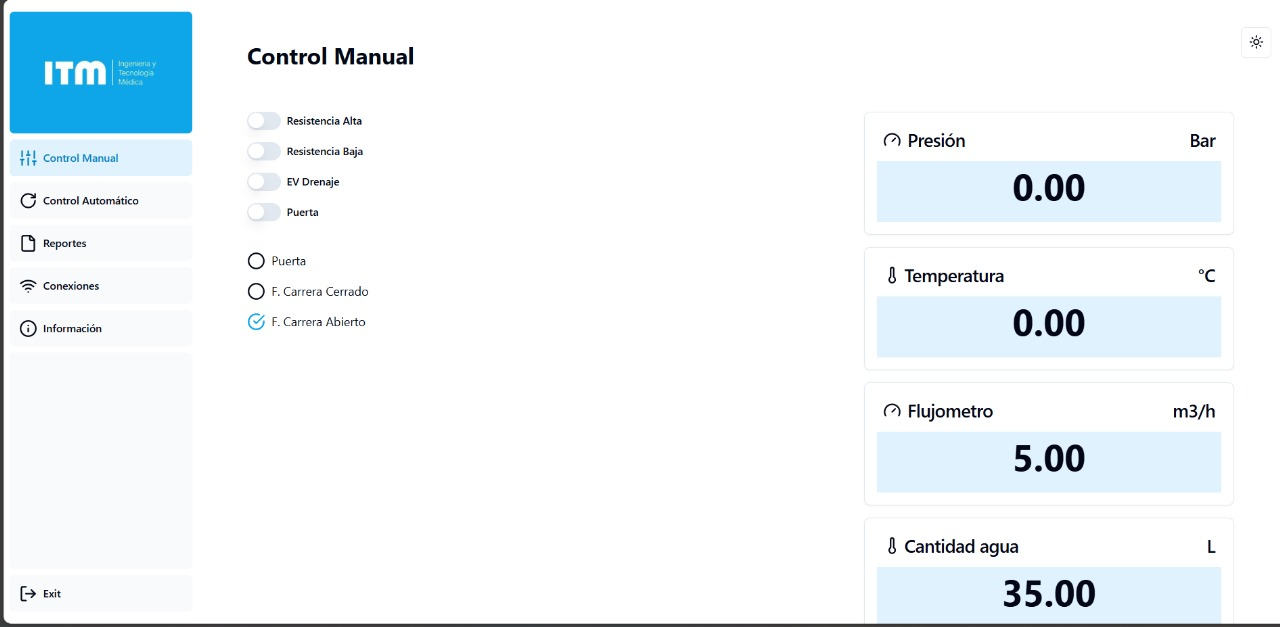
\includegraphics[width=0.9\columnwidth]{Figuras/8.jpg}}\\
    \centering{\textbf{Fuente:} Elaboración propia (2024)} % Fuente
    \label{fig:man}
\end{figure}

\textbf{Control Automático:} La página presenta las gráficas de presión y temperatura para poder observar los valores en tiempo real de la autoclave Figura \ref{fig:aut}.
\begin{figure}[!htb]
    \centering
    \caption{Control Automático} % Título de figura
    {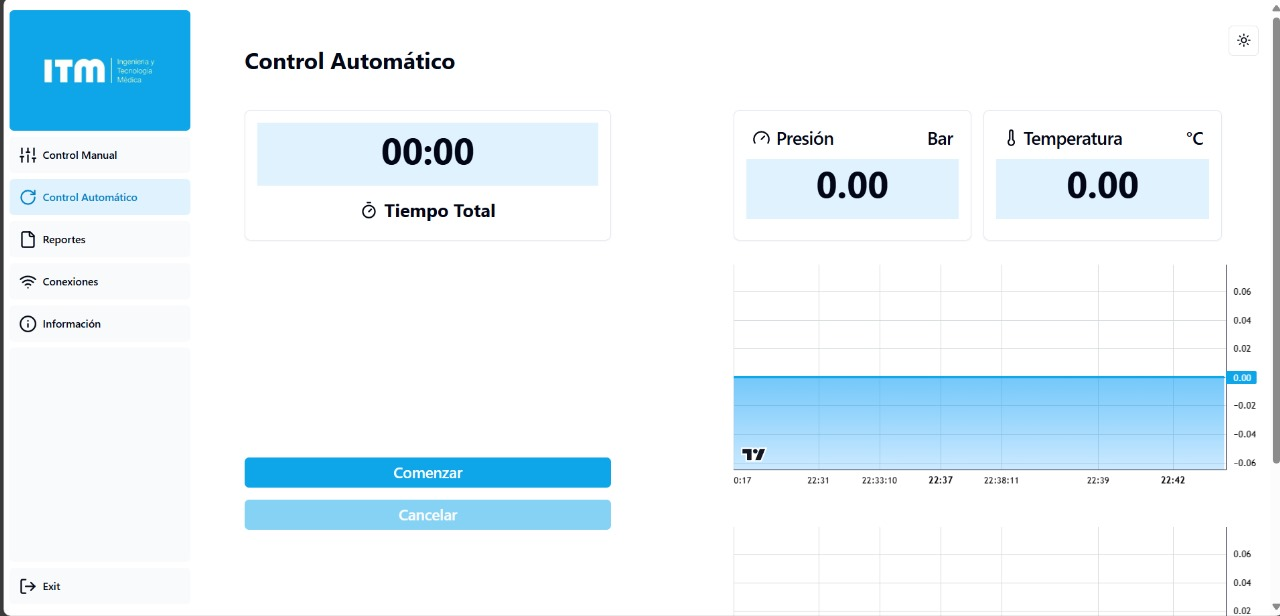
\includegraphics[width=0.9\columnwidth]{Figuras/5.jpg}}\\
    \centering{\textbf{Fuente:} Elaboración propia (2024)} % Fuente
    \label{fig:aut}
\end{figure}

\textbf{Reportes:} Como se observa en la Figura\ref{fig:rep} esta presenta datos históricos de ciclos de la autoclave.
\begin{figure}[!htb]
    \centering
    \caption{Reportes} % Título de figura
    {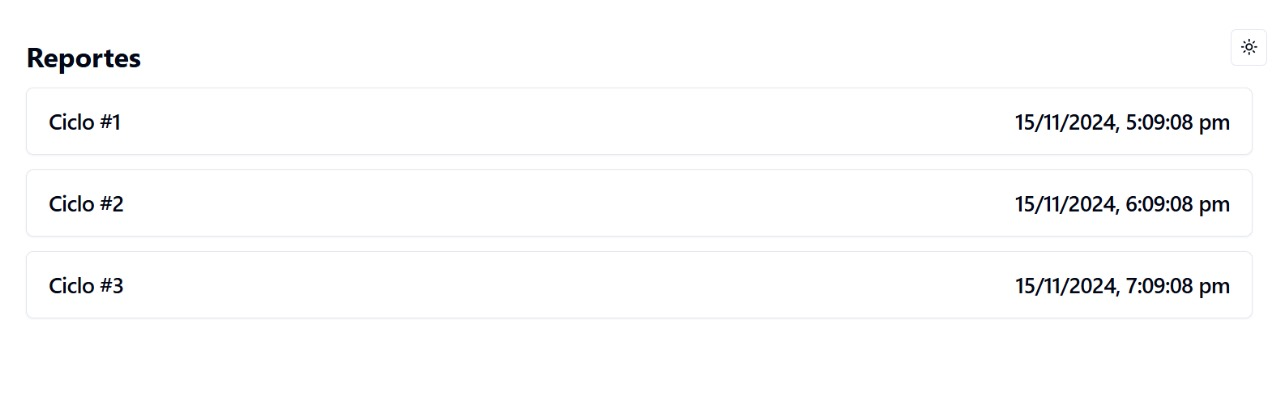
\includegraphics[width=0.9\columnwidth]{Figuras/10.jpg}}\\
    \centering{\textbf{Fuente:} Elaboración propia (2024)} % Fuente
    \label{fig:rep}
\end{figure}
\newpage
\textbf{Conexiones e información:} Finalmente en estas páginas obtenemos información a cerca de la autoclave y su red \acrshort{wifi}, como también se tiene la posibilidad de actualizar estos datos Figura\ref{fig:inf}.
\begin{figure}[hpt]
    \centering
    % Título de figura
    \caption{Páginas de información}
        % imagen 1
        \subfloat[Conexiones]{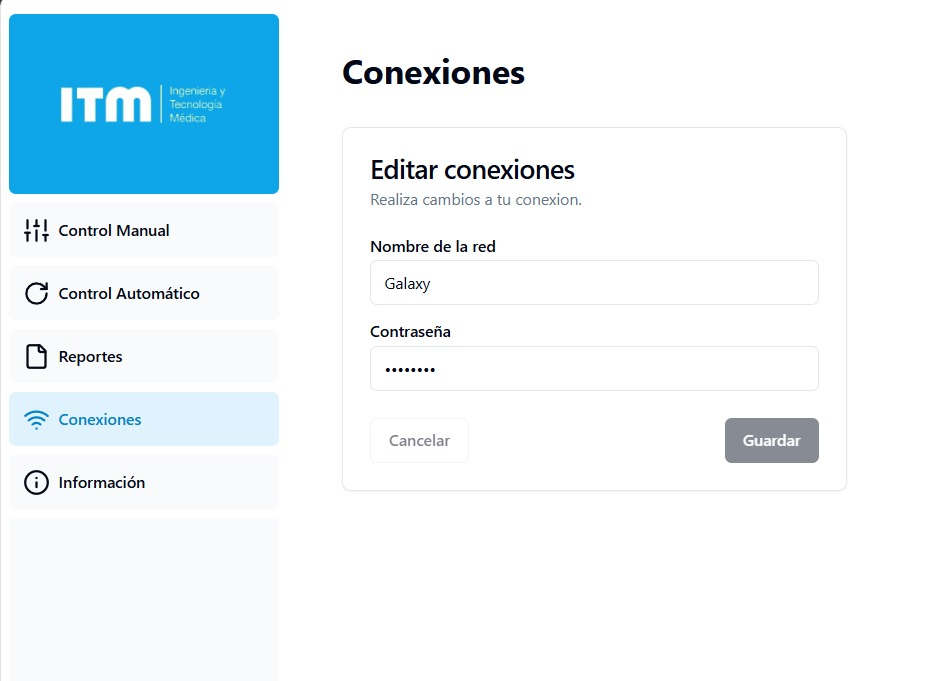
\includegraphics[width=0.5\columnwidth]{Figuras/2.jpg}}
        % separaciones | agregar una de las opciones entre cada par de imágenes
            \qquad      % figuras en la misma linea
            %\par        % siguiente línea
        % imagen 2
        \subfloat[Información]{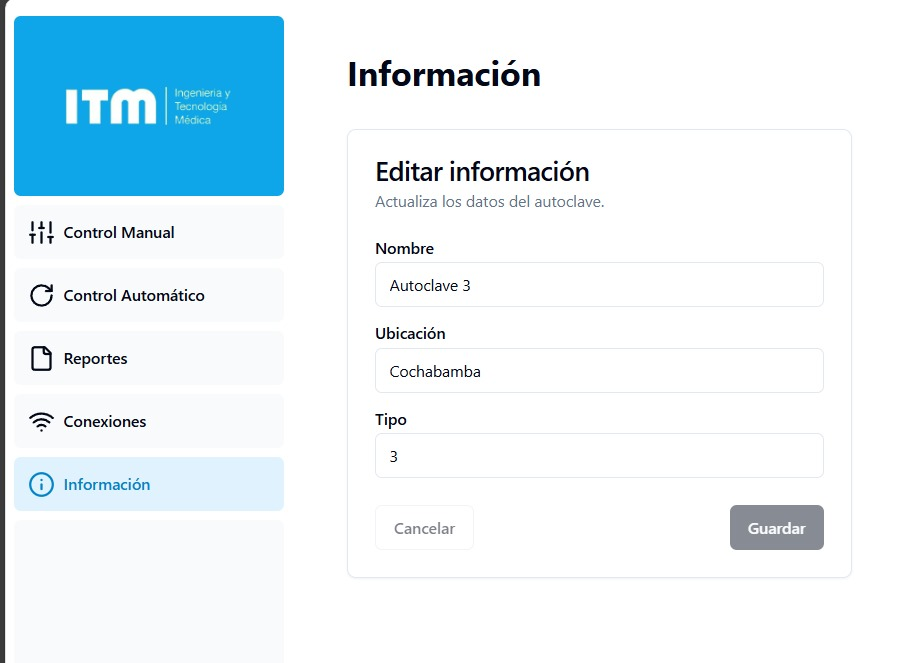
\includegraphics[width=0.5\columnwidth]{Figuras/3.jpg}}\\
    \centering{\textbf{Fuente:} Elaboración propia (2024)}
    \label{fig:inf}
\end{figure}

\subsubsection{Implementación mecánica}
La carcasa de la placa del sistema de monitoreo es impresa en 3d con el material de \acrshort{pla}, posteriormente se adjunta cada pieza en conjunto con la placa \acrshort{pcb} como se puede observar en la Figura \ref{fig:car}.
\begin{figure}[!htb]
    \centering
    \caption{Prototipo final} % Título de figura
    {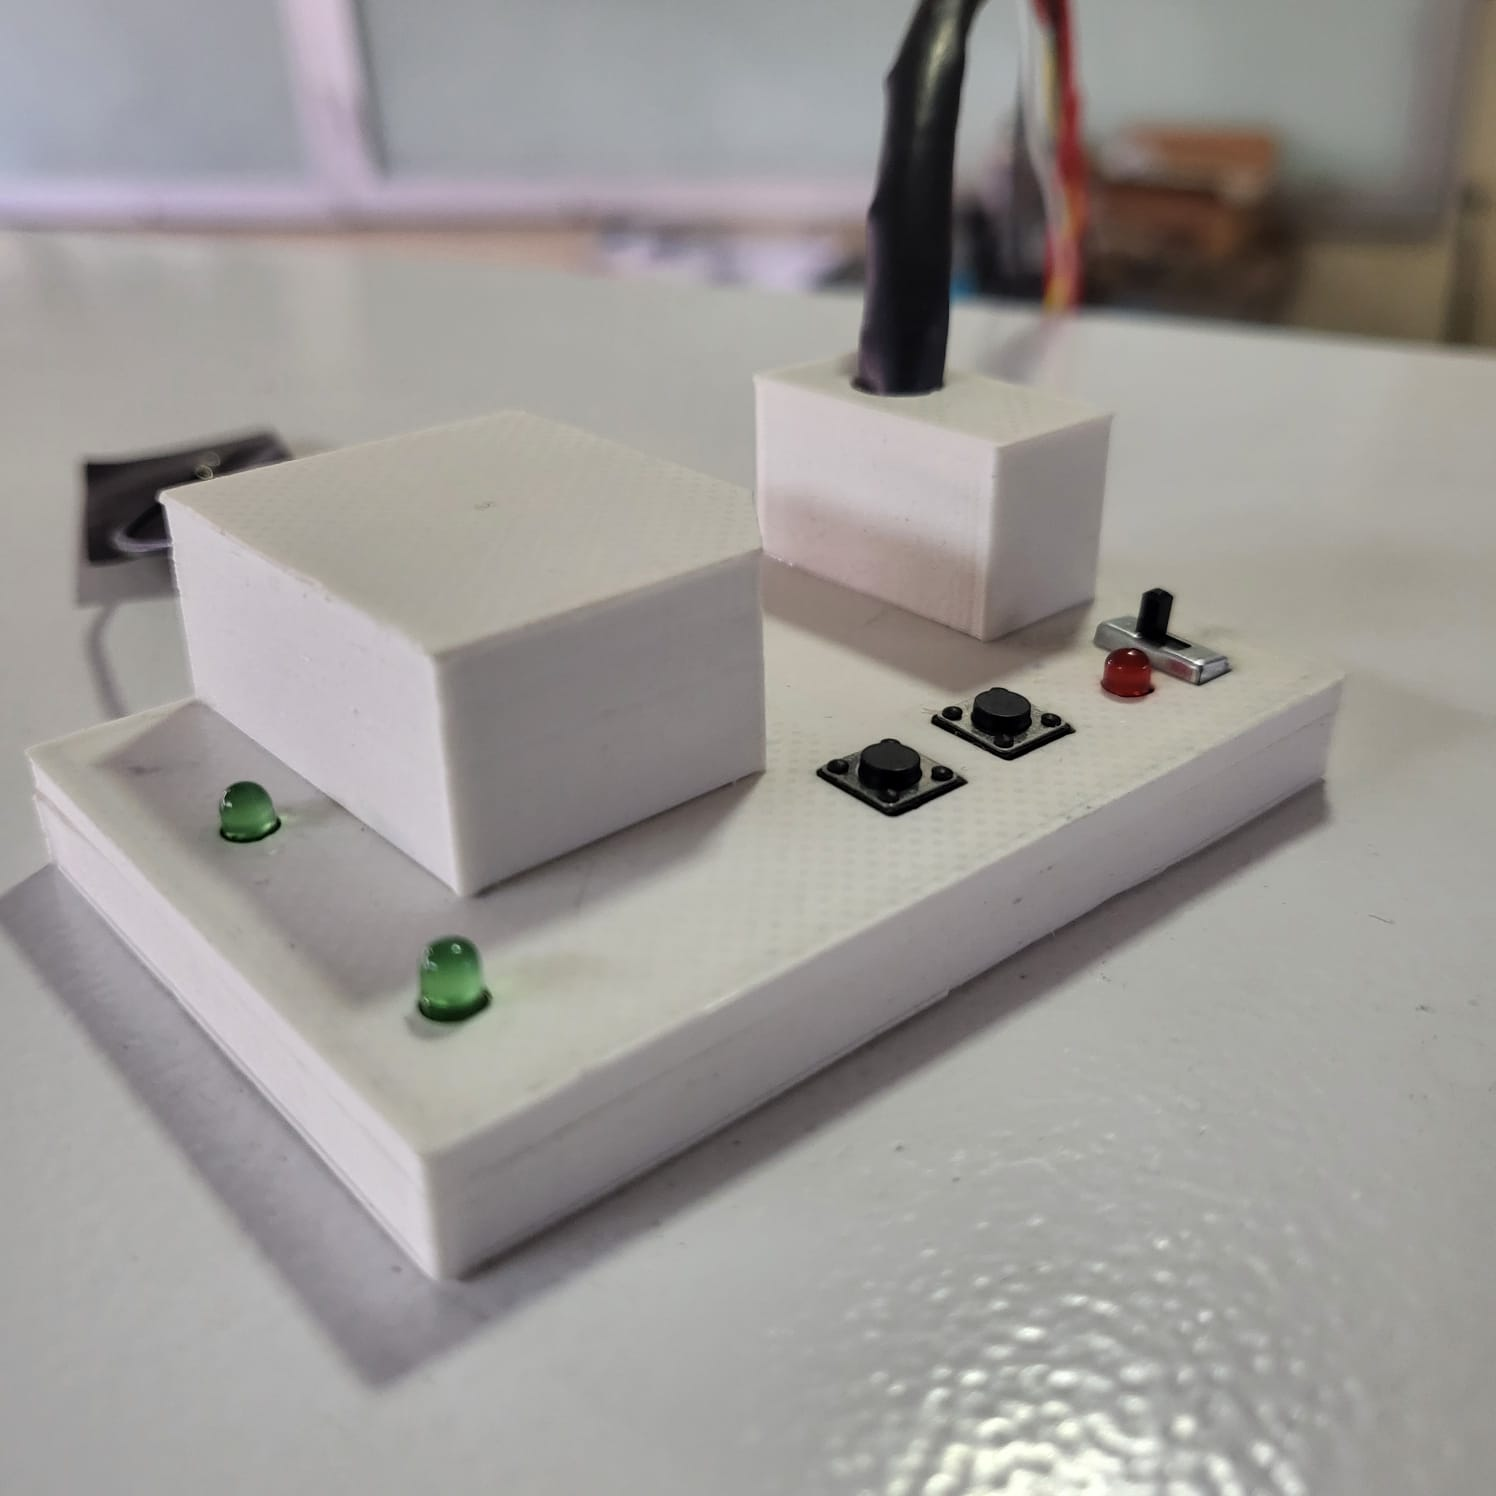
\includegraphics[width=0.6\columnwidth]{Figuras/implementacion/mec1.jpg}}\\
    \centering{\textbf{Fuente:} Elaboración propia (2024)} % Fuente
    \label{fig:car}
\end{figure}

Finalmente se ensambla el prototipo en la puerta de la autoclave Figura \ref{fig:fin}, puesto que no se sufre de interferencia en esa área.
\begin{figure}[hpt]
    \centering
    % Título de figura
    \caption{Ensamblaje en la puerta}
        % imagen 1
        \subfloat[Vista frontal]{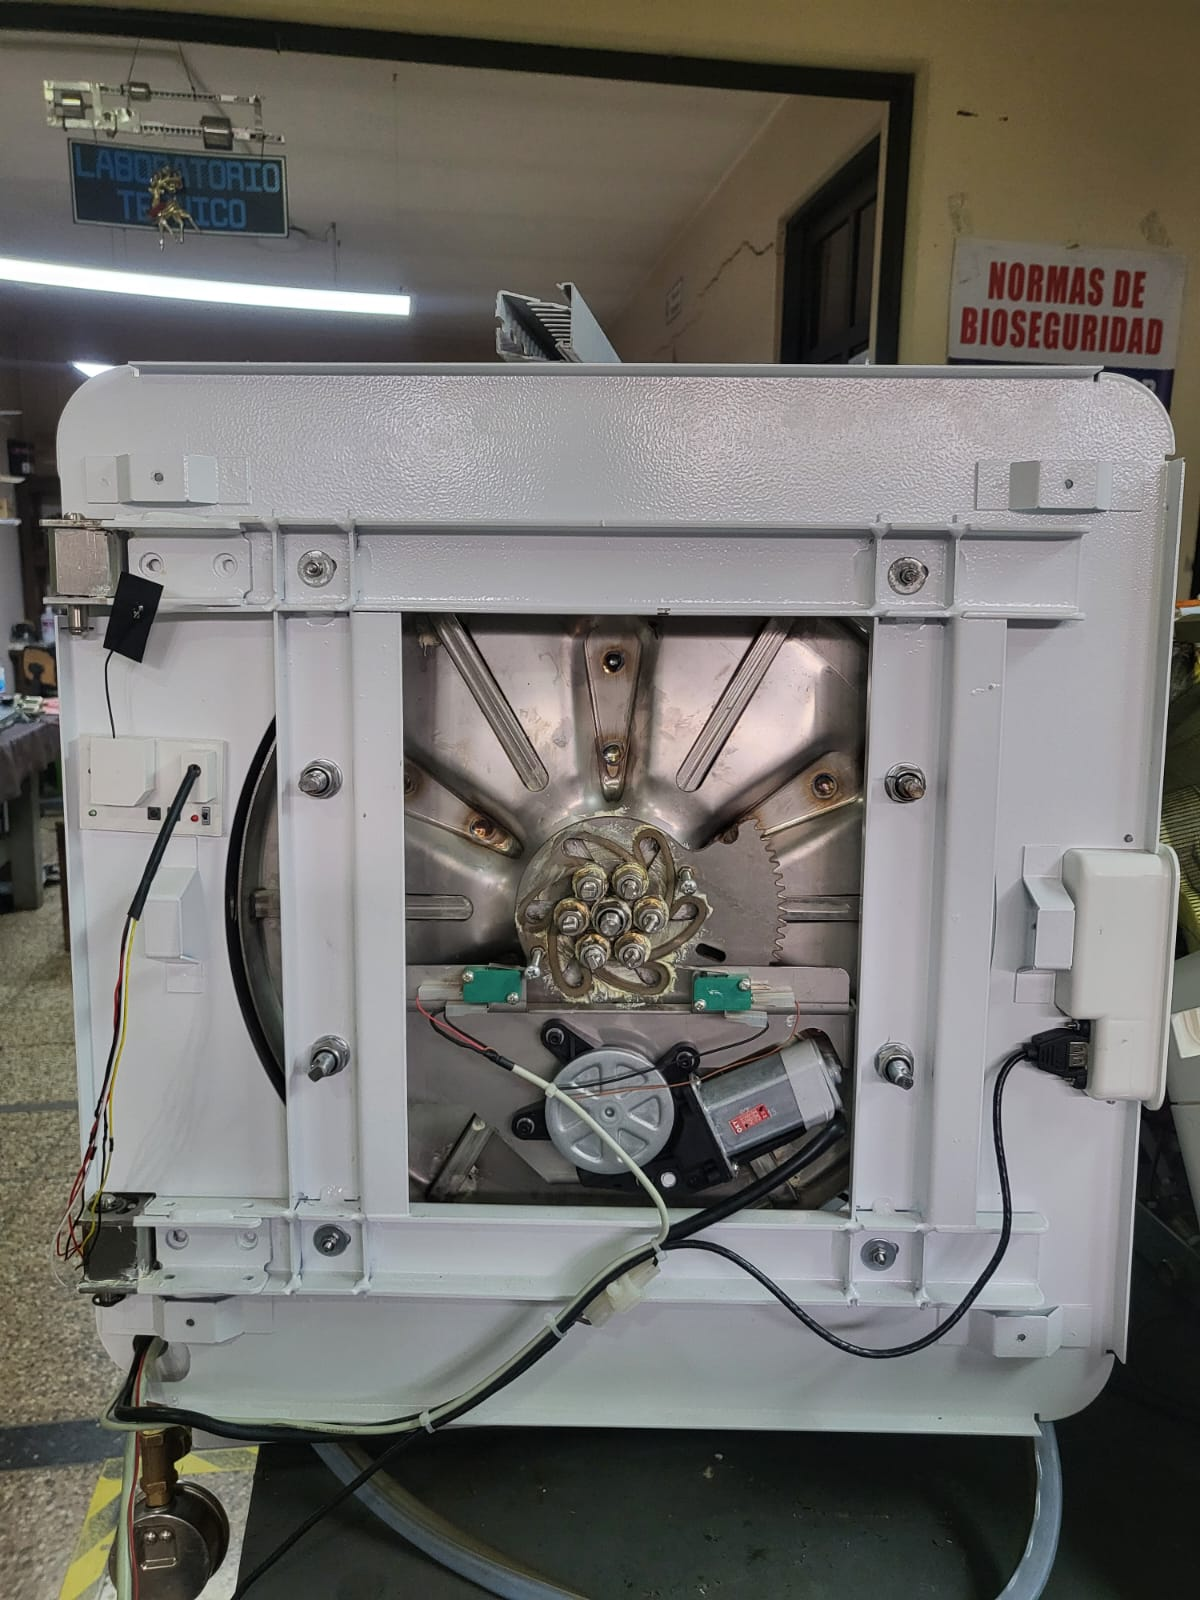
\includegraphics[width=0.5\columnwidth]{Figuras/implementacion/mec2.jpg}}
        % separaciones | agregar una de las opciones entre cada par de imágenes
            \qquad      % figuras en la misma linea
            %\par        % siguiente línea
        % imagen 2
        \subfloat[Vista general]{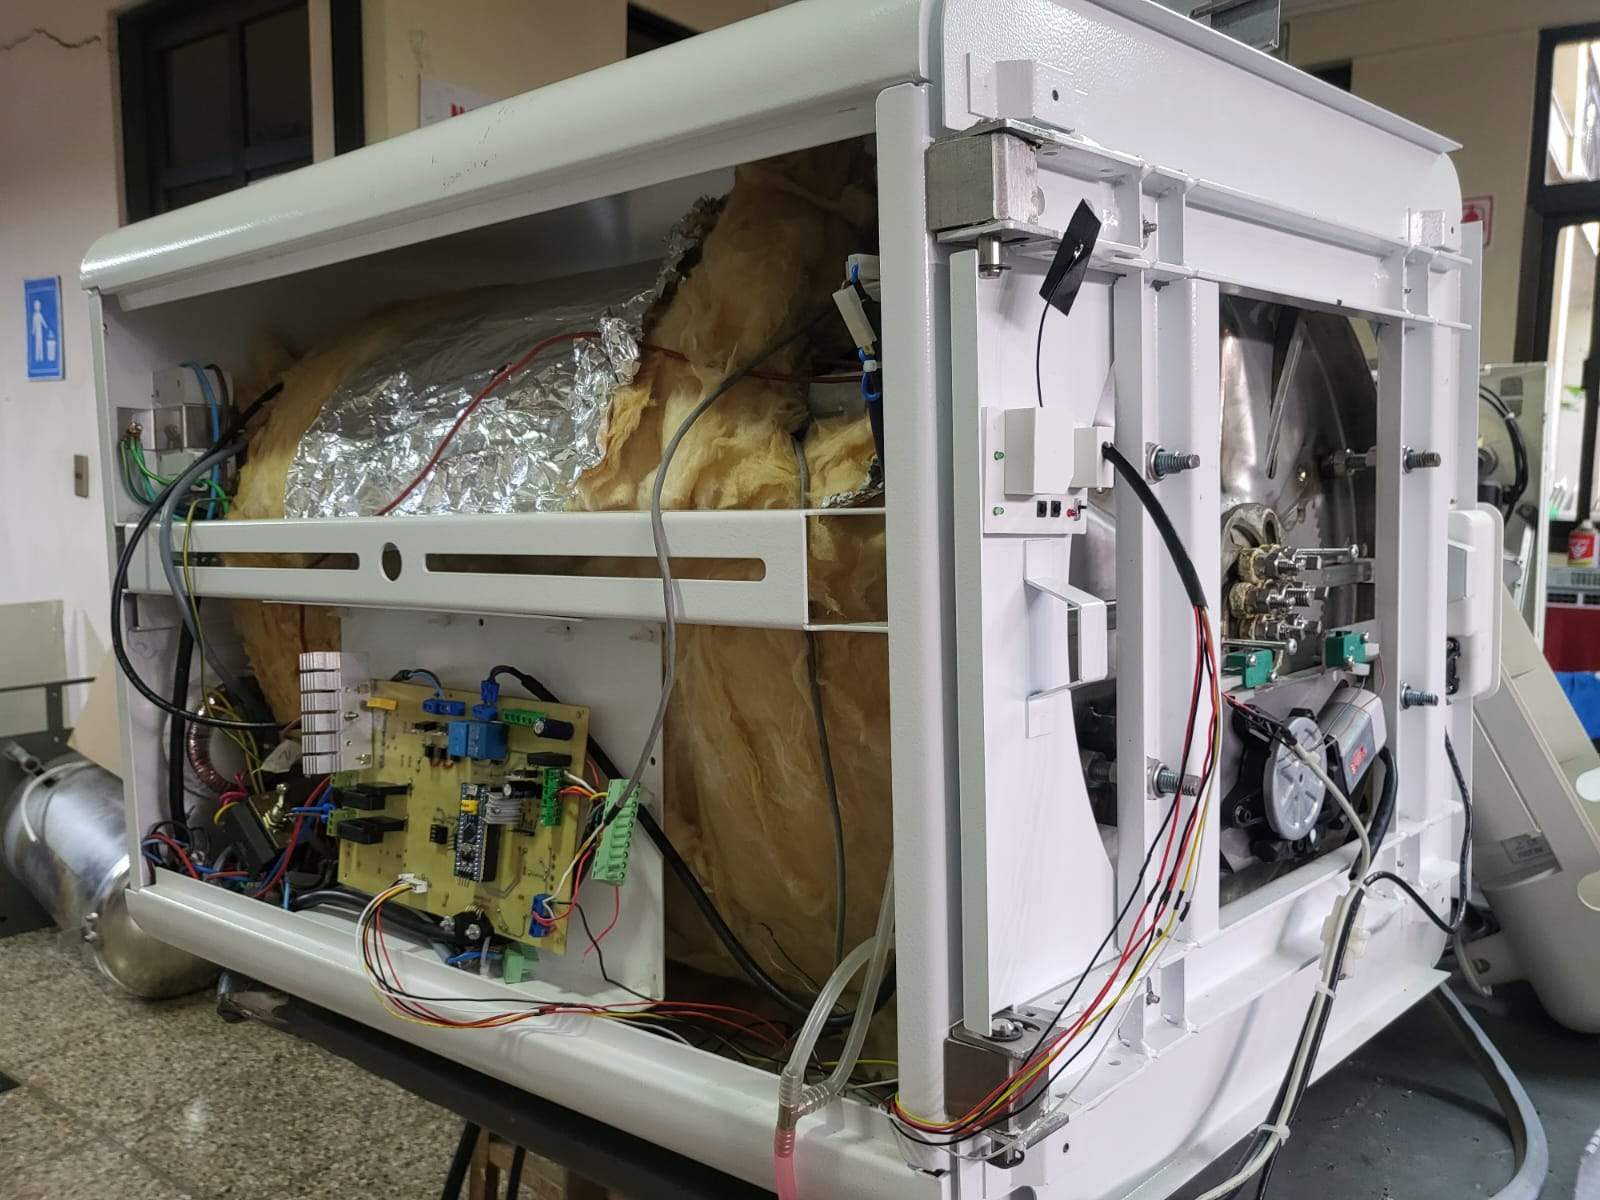
\includegraphics[width=0.5\columnwidth]{Figuras/implementacion/mec3.jpg}}\\
    \centering{\textbf{Fuente:} Elaboración propia (2024)}
    \label{fig:fin}
\end{figure}
\newpage
\subsection{Resultados}
Realizando las debidas pruebas en ambientes controlados, se puede verificar que se garantiza la fiabilidad del envío y recolección de datos a partir de la placa de control de la autoclave hasta el almacenamiento en la base de datos. Para ello se puede observar las siguientes gráficas, donde se muestra la cantidad de datos enviados, sesiones iniciadas y suscripciones a tópicos creados en las Figuras \ref{fig:res1},\ref{fig:res2}.
\begin{figure}[hpt]
    \centering
    % Título de figura
    \caption{Resultados de clientes}
        % imagen 1
        \subfloat[Sesiones]{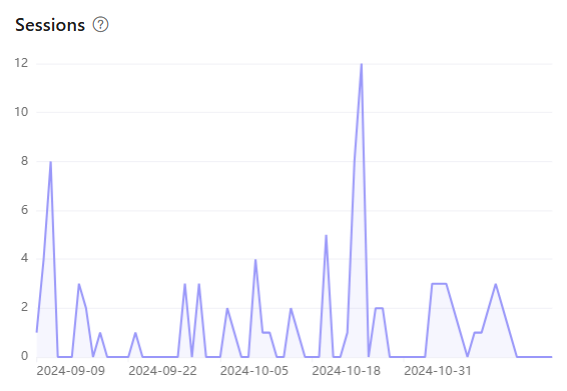
\includegraphics[width=0.6\columnwidth]{Figuras/res1.png}}
        % separaciones | agregar una de las opciones entre cada par de imágenes
            %\qquad      % figuras en la misma linea
            \par        % siguiente línea
        % imagen 2
        \subfloat[Suscripciones]{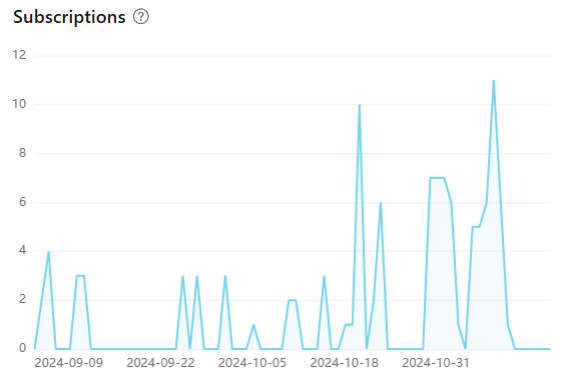
\includegraphics[width=0.6\columnwidth]{Figuras/res2.png}}\\
    \centering{\textbf{Fuente:} Elaboración propia (2024)}
    \label{fig:res1}
\end{figure}
\newpage
\begin{figure}[hpt]
    \centering
    % Título de figura
    \caption{Resultados de datos}
        % imagen 1
        \subfloat[Mensajes]{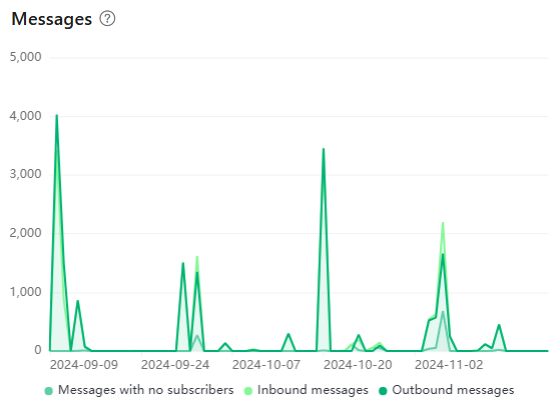
\includegraphics[width=0.6\columnwidth]{Figuras/res3.png}}
        % separaciones | agregar una de las opciones entre cada par de imágenes
            %\qquad      % figuras en la misma linea
            \par        % siguiente línea
        % imagen 2
        \subfloat[Paquetes]{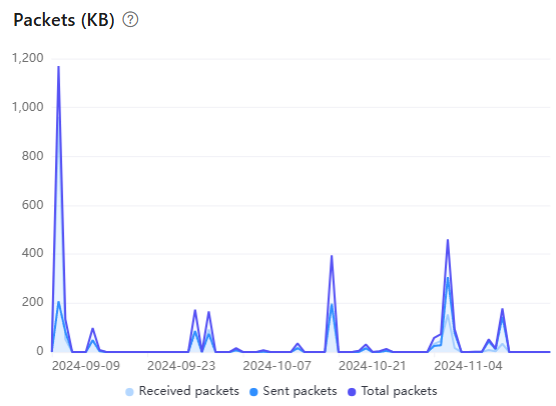
\includegraphics[width=0.6\columnwidth]{Figuras/res4.png}}\\
    \centering{\textbf{Fuente:} Elaboración propia (2024)}
    \label{fig:res2}
\end{figure}

En las figuras se puede apreciar la cantidad de mensajes recibido con la cantidad de paquetes de memoria, a la vez se puede verificar la conexión de clientes por \acrshort{mqtt} y su tiempo de conexión.